%! Mode:: "TeX:UTF-8"
%! TEX program = xelatex
\PassOptionsToPackage{quiet}{xeCJK}
\documentclass[withoutpreface,bwprint]{cumcmthesis}
\usepackage{etoolbox}
\BeforeBeginEnvironment{tabular}{\zihao{-5}}
\usepackage[numbers,sort&compress]{natbib}  % 文献管理宏包
\usepackage[framemethod=TikZ]{mdframed}  % 框架宏包
\usepackage{url}  % 网页链接宏包
\usepackage{subcaption}  % 子图宏包
\newcolumntype{C}{>{\centering\arraybackslash}X}
\newcolumntype{R}{>{\raggedleft\arraybackslash}X}
\newcolumntype{L}{>{\raggedright\arraybackslash}X}

\usepackage{multirow}
\usepackage{array}

\title{全国大学生数学建模竞赛论文模板}  % 论文标题
\tihao{}  % 题号
\baominghao{}  % 报名号
\schoolname{}  % 学校
\membera{}  % 队员a
\memberb{}  % 队员b
\memberc{}  % 队员c
\supervisor{}  % 指导老师
\yearinput{}
\monthinput{}
\dayinput{}

%%%%%%%%%%%%%%%%%%%%%%%%%%%%%%%%%%%%%%%%%%%%%%%%%%%%%%%%%%%%%
%% 正文
\begin{document}
\begin{samepage}
\begin{center}
\renewcommand{\arraystretch}{2}
\begin{tabular}{|>{\centering\arraybackslash}m{0.13\textwidth}
                |>{\centering\arraybackslash}m{0.65\textwidth}
                |>{\centering\arraybackslash}m{0.17\textwidth}|}
    \hline
    \songti 所属类别
    & \multirow{2}{*}{\centering\songti\zihao{4} \textbf{2024年“华数杯”全国大学生数学建模竞赛}}
    & \songti 参赛编号 \\
    \cline{1-1} \cline{3-3}
    \songti 本科组 & & CM2400947 \\
    \hline
\end{tabular}
\end{center}

\maketitle

\begin{abstract}
    母亲的身心健康对婴儿的早期成长和发展具有重要影响。已有研究表明,母亲的身体状况以及心理健康(如压力、抑郁、焦虑等)不仅关系到婴儿的生理健康,还会影响婴儿的认知、情感、社会行为等多方面成长。婴儿的行为特征和睡眠质量常常作为衡量婴儿发展状况的重要指标。基于这方面的专业背景,本文对相关影响机制进行了研究与建模。
    
    \textbf{对于问题一,}本文通过分析390名婴儿及其母亲的身体和心理相关指标数据,研究了母亲因素对婴儿行为特征和睡眠质量的影响关系。
    
    \textbf{对于问题二,}基于婴儿行为问卷,将婴儿行为特征划分为安静型、中等型和矛盾型,建立了行为特征与母亲身体、心理指标之间的数学关系模型,并利用该模型预测了20组缺失婴儿行为类型。
    
    \textbf{对于问题三,}建立了CBTS、EPDS、HADS评分与治疗费用的关联模型,针对编号238的矛盾型婴儿,分析通过最小治疗费用使其行为特征由矛盾型转变为中等型和安静型的策略及调整路径。
    
    \textbf{对于问题四,}选取婴儿睡眠的多项指标,综合评判睡眠质量,并建立母亲各项指标与婴儿综合睡眠质量的关联模型,进而预测缺失数据婴儿的睡眠类别。
    
    最后,结合模型结果,对如何提升238号婴儿的睡眠质量等级为优提出了具体的治疗方案和优化建议。
    
    \keywords{母亲心理健康\quad  婴儿成长\quad  行为特征\quad  睡眠质量 \quad 数学建模}
    \end{abstract}
\end{samepage}
%%%%%%%%%%%%%%%%%%%%%%%%%%%%%%%%%%%%%%%%%%%%%%%%%%%%%%%%%%%%% 

% \tableofcontents  % 目录
% \newpage

%%%%%%%%%%%%%%%%%%%%%%%%%%%%%%%%%%%%%%%%%%%%%%%%%%%%%%%%%%%%%  
\section{问题重述}
\subsection{问题背景}
问题背景

%%%%%%%%%%%%%%%%%%%%%%%%%%%%%%%%%%%%%%%%%%%%%%%%%%%%%%%%%%%%% 

\subsection{问题要求}

\textbf{问题1}  

\textbf{问题2}  

\textbf{问题3} 

\textbf{问题4}  

%%%%%%%%%%%%%%%%%%%%%%%%%%%%%%%%%%%%%%%%%%%%%%%%%%%%%%%%%%%%% 

\section{问题分析}
\subsection{问题一分析}
对于问题一,

\subsection{问题二分析}	
对于问题二,

\subsection{问题三分析}
对于问题三,

\subsection{问题四分析}
对于问题四,

%%%%%%%%%%%%%%%%%%%%%%%%%%%%%%%%%%%%%%%%%%%%%%%%%%%%%%%%%%%%% 

\section{模型假设}

为简化问题,本文做出以下假设:

\begin{itemize}[itemindent=2em]
\item 假设1
\item 假设2
\item 假设3
\end{itemize}

%%%%%%%%%%%%%%%%%%%%%%%%%%%%%%%%%%%%%%%%%%%%%%%%%%%%%%%%%%%%% 

\section{符号说明}
\begin{table}[H]
\centering
\begin{tabularx}{\textwidth}{CLC}
\toprule
符号    & 说明    & 单位 \\
\midrule
$m     $& 质量 & $kg$ \\
$V     $& 体积 & $m^3$ \\
\bottomrule
\end{tabularx}
\label{tab:符号说明}
\end{table}


%%%%%%%%%%%%%%%%%%%%%%%%%%%%%%%%%%%%%%%%%%%%%%%%%%%%%%%%%%%%% 

\section{问题一的模型的建立和求解}


\subsection{数据预处理与特征工程}
高质量的数据是构建有效模型的基础。针对原始数据集,我们进行了以下关键的数据预处理和特征工程步骤:

\subsubsection{睡眠时间格式转换}
原始数据中婴儿“整晚睡眠时间”以“HH:MM”字符串格式记录,且存在“99:99”等异常值。我们将其转换统一为浮点数表示的小时数,并对异常值进行处理,通常将其视为缺失值或根据业务逻辑进行填充。
$$ \text{时间}_{\text{小时}} = \text{小时} + \frac{\text{分钟}}{60} $$
此转换确保了睡眠时间数据的数值化和可计算性。

\subsubsection{分类变量编码与映射}
数据集中包含婚姻状况、教育程度、分娩方式、婴儿性别、入睡方式和婴儿行为特征等分类变量。为使其能够被回归模型处理,我们进行了以下操作:
\begin{itemize}
    \item \textbf{数值映射为标签}:将原始的数值编码(如1、2、3等)映射为更具可读性的类别标签(如“未婚”、“已婚”;“哄睡法”、“自主入睡”)。
    \item \textbf{独热编码 (One-Hot Encoding)}:对于无序的分类变量,如入睡方式、教育程度等,采用独热编码将其转换为二元(0/1)指示变量。这避免了将分类变量误解释为有序数值,并消除了因任意数值赋值而引入的潜在偏差。例如,教育程度的“研究生”类别将被转换为一个独立的二元特征。
\end{itemize}
婴儿行为特征作为因变量,被映射为数值(如安静型=0,中等型=1,矛盾型=2),以适应多项逻辑回归模型的输入要求。

\subsubsection{数值型特征标准化}
对于母亲年龄、妊娠时间、CBTS、EPDS、HADS等数值型预测变量,我们采用标准差标准化(Z-score normalization)处理。
$$ X' = \frac{X - \mu}{\sigma} $$
其中,$X$ 是原始特征值,$\mu$ 是特征的均值,$\sigma$ 是特征的标准差。标准化后的特征均值为0,标准差为1。此步骤有助于:
\begin{itemize}
    \item 消除不同特征量纲和取值范围差异带来的影响,确保模型优化过程中所有特征得到同等重视。
    \item 加速模型收敛,尤其对于基于梯度下降的优化算法(如逻辑回归)。
    \item 提高模型的可解释性和稳定性,避免某些特征因数值过大而主导模型。
\end{itemize}
这些预处理步骤共同确保了数据的规范性、一致性和可用性,为后续的模型构建奠定了坚实基础。

\subsection{探索性数据分析 (EDA) 结果}
在模型构建之前,我们进行了全面的探索性数据分析,以揭示数据内部的结构、变量分布以及变量间的潜在关联。

\subsubsection{变量分布特征}
我们首先分析了关键变量的分布情况。
\begin{itemize}
    \item \textbf{母亲心理指标分布}:如图\ref{fig:psychological_indicators_distribution}所示,CBTS、EPDS和HADS得分均呈右偏分布,表明大多数母亲心理状况良好,但存在一定比例的母亲有心理健康问题。
    \item \textbf{婴儿睡眠质量指标分布}:如图\ref{fig:sleep_quality_distribution}所示,婴儿整晚睡眠时间主要集中在10-12小时,符合婴儿的正常睡眠需求;睡醒次数主要集中在0-2次,但也存在少数婴儿睡醒次数较多。
    \item \textbf{婴儿行为特征分布}:如图\ref{fig:baby_behavior_distribution}所示,样本中中等型婴儿占比最高(57.7\%),其次为安静型(30.8\%),矛盾型婴儿占比最低(11.5\%),存在明显的类别不平衡。
\end{itemize}

\begin{figure}[htbp]
    \centering
    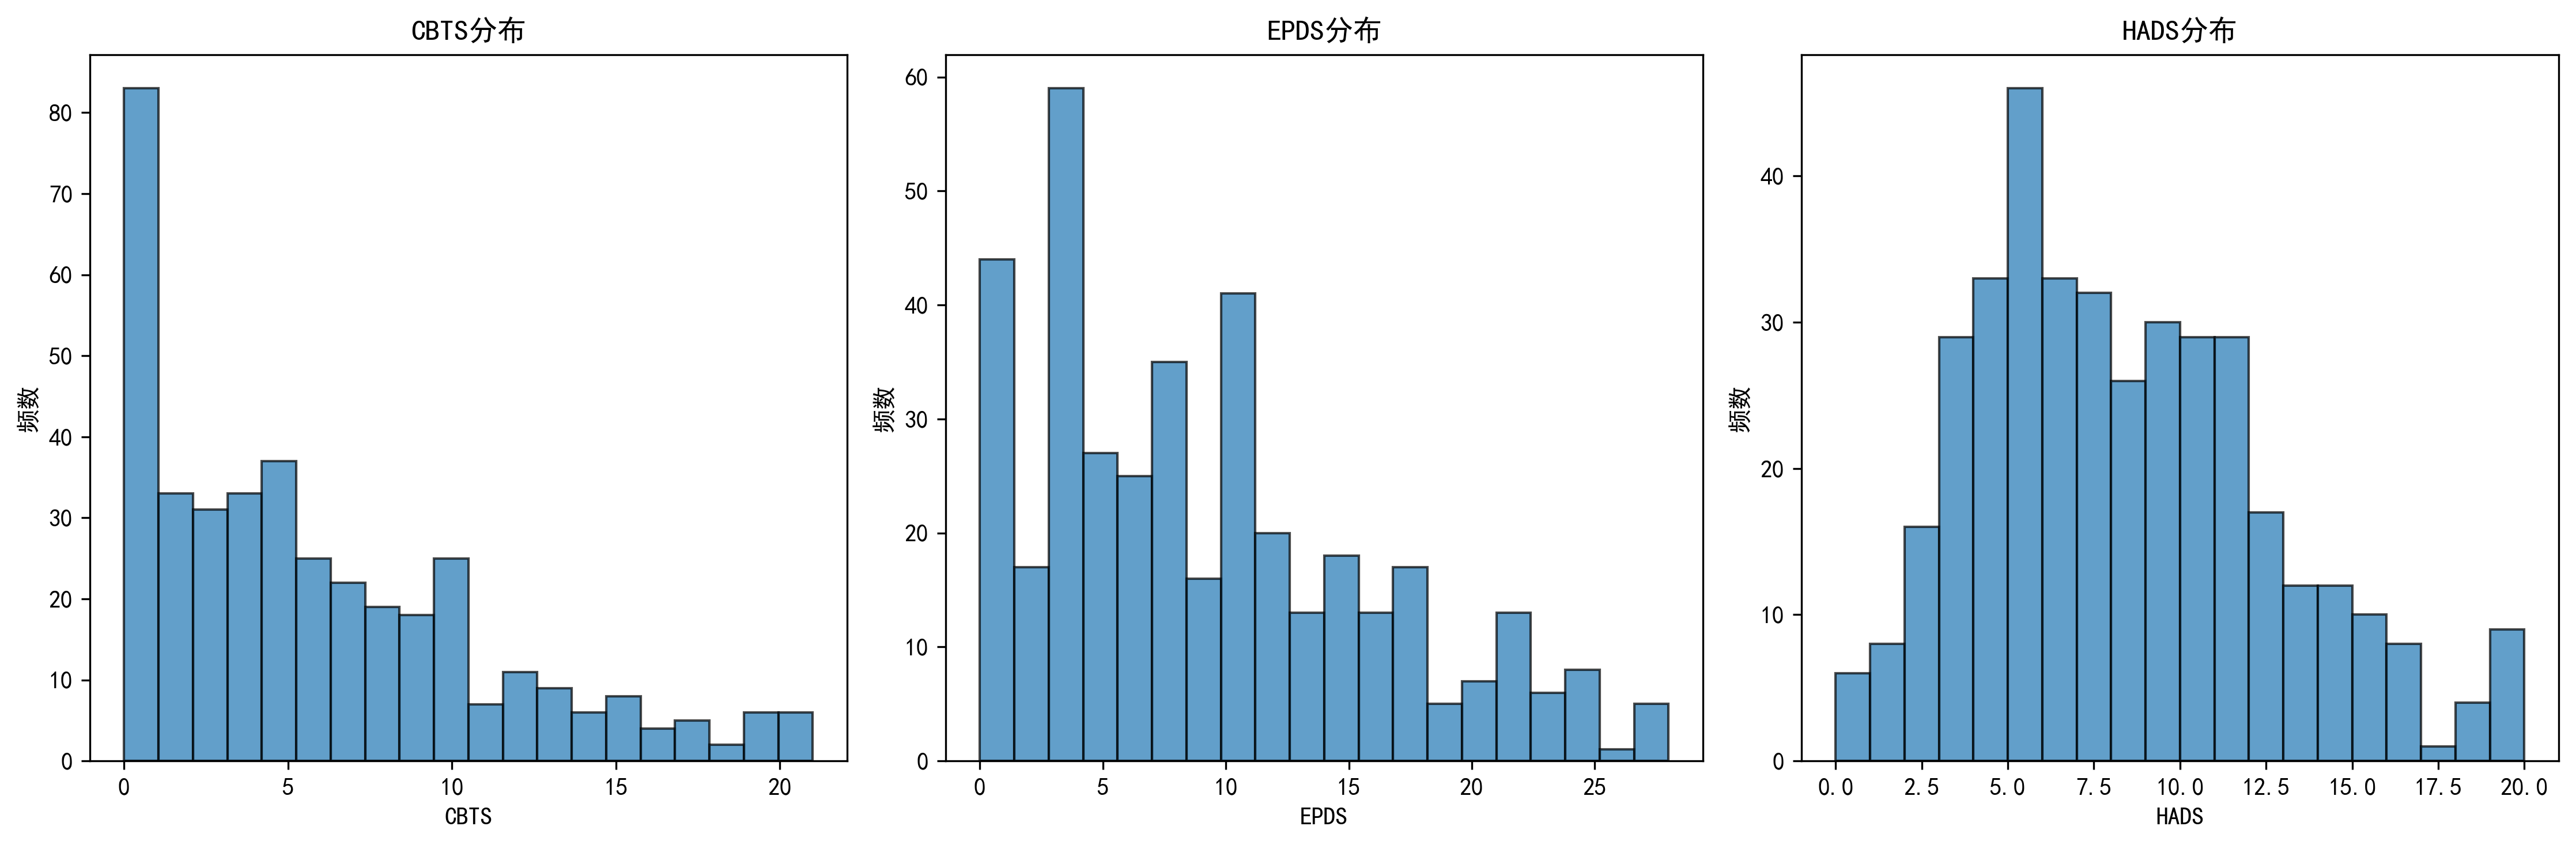
\includegraphics[width=0.9\textwidth]{figures/psychological_indicators_distribution.png}
    \caption{母亲心理指标分布}
    \label{fig:psychological_indicators_distribution}
\end{figure}

\begin{figure}[htbp]
    \centering
    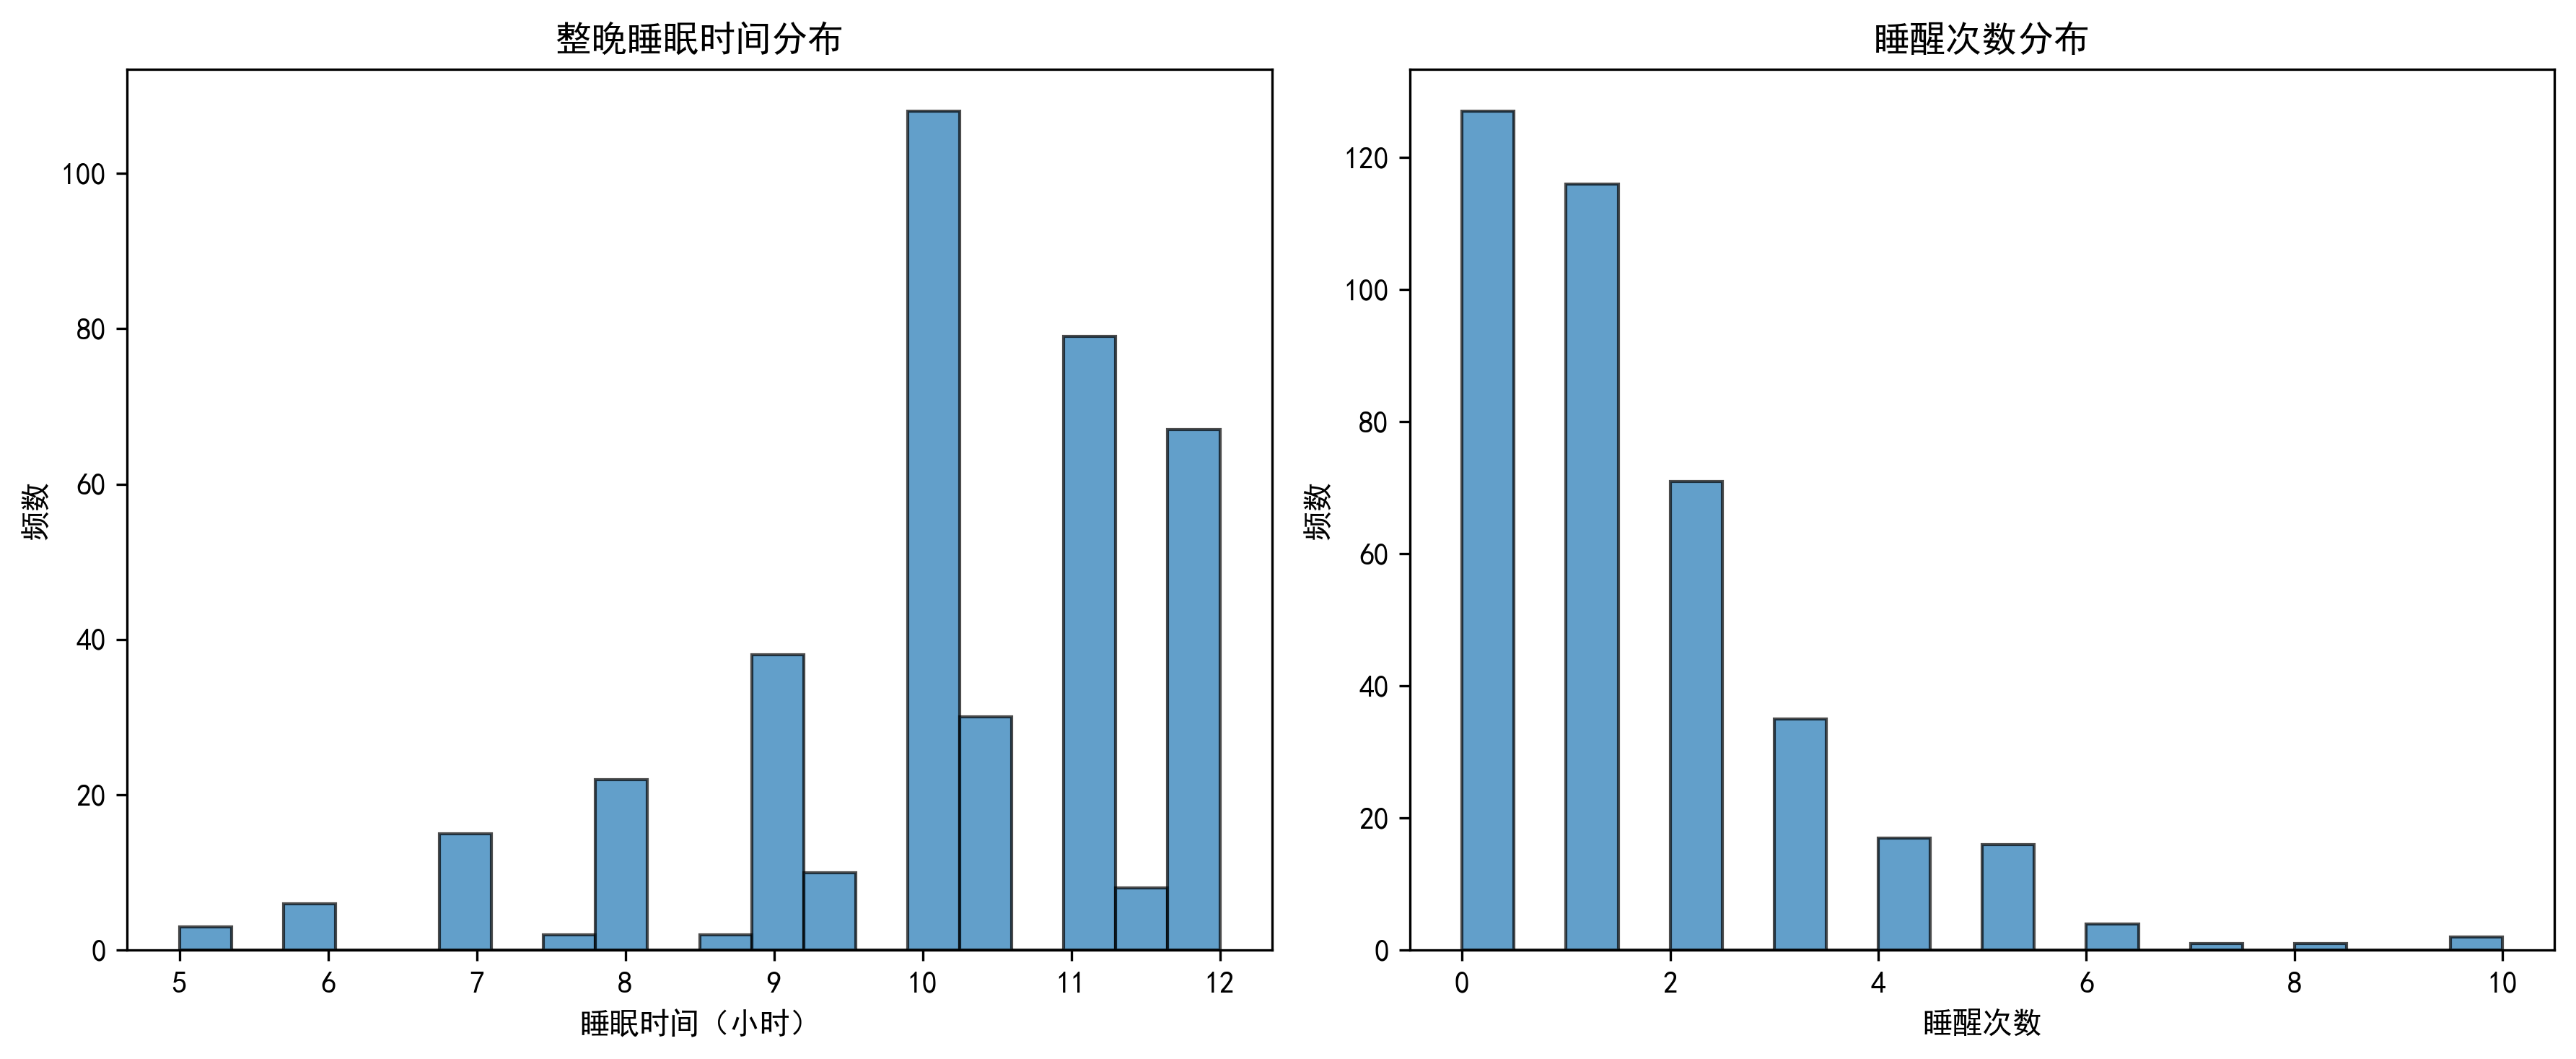
\includegraphics[width=0.8\textwidth]{figures/sleep_quality_distribution.png}
    \caption{睡眠质量指标分布}
    \label{fig:sleep_quality_distribution}
\end{figure}

\begin{figure}[htbp]
    \centering
    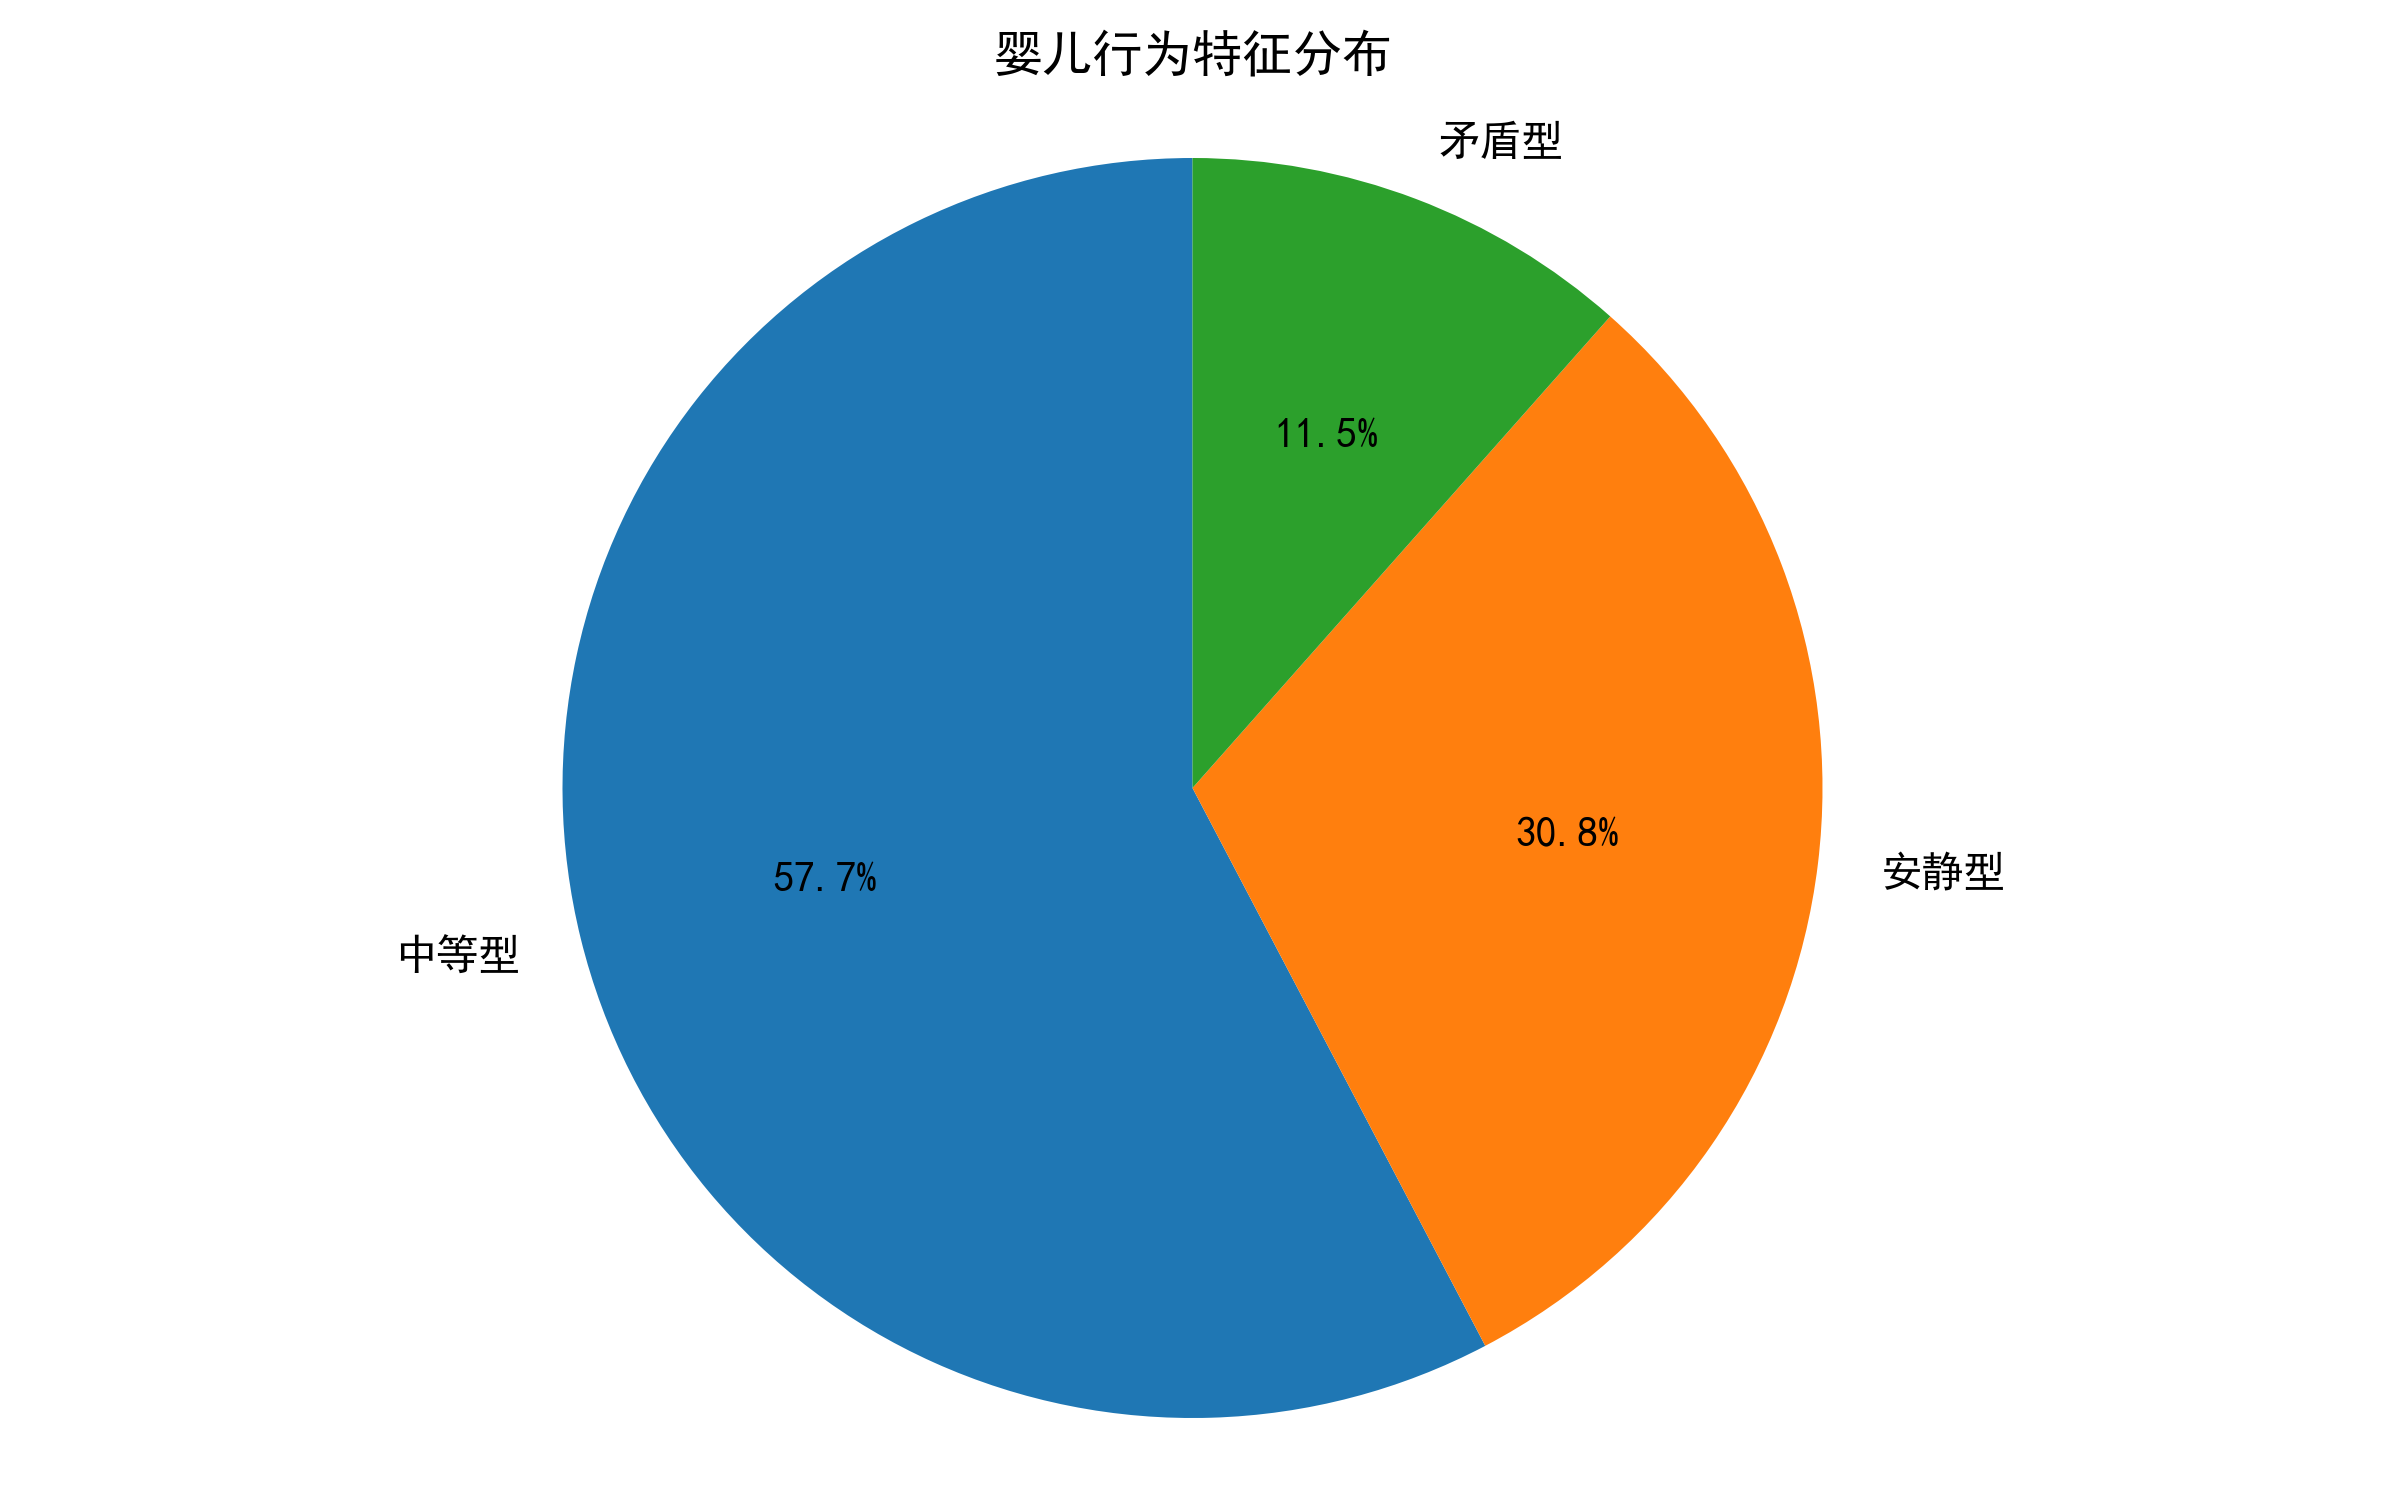
\includegraphics[width=0.5\textwidth]{figures/baby_behavior_distribution.png}
    \caption{婴儿行为特征分布}
    \label{fig:baby_behavior_distribution}
\end{figure}

\subsubsection{相关性分析}
我们计算了数值型变量间的皮尔逊相关系数,并生成相关性热力图(如图\ref{fig:correlation_heatmap}所示)。
\begin{itemize}
    \item \textbf{母亲心理指标之间存在强相关性}:EPDS与HADS相关系数高达0.79,CBTS与EPDS为0.78,CBTS与HADS为0.69。这表明抑郁、焦虑和创伤后应激障碍往往同时出现,提示在临床干预中应综合考虑。
    \item \textbf{母亲心理指标与婴儿睡眠质量的负相关}:母亲心理指标(CBTS、EPDS、HADS)与婴儿整晚睡眠时间呈弱到中等程度的负相关,与睡醒次数呈正相关。这初步揭示了母亲心理压力越大,婴儿睡眠质量可能越差的规律。
\end{itemize}

\begin{figure}[htbp]
    \centering
    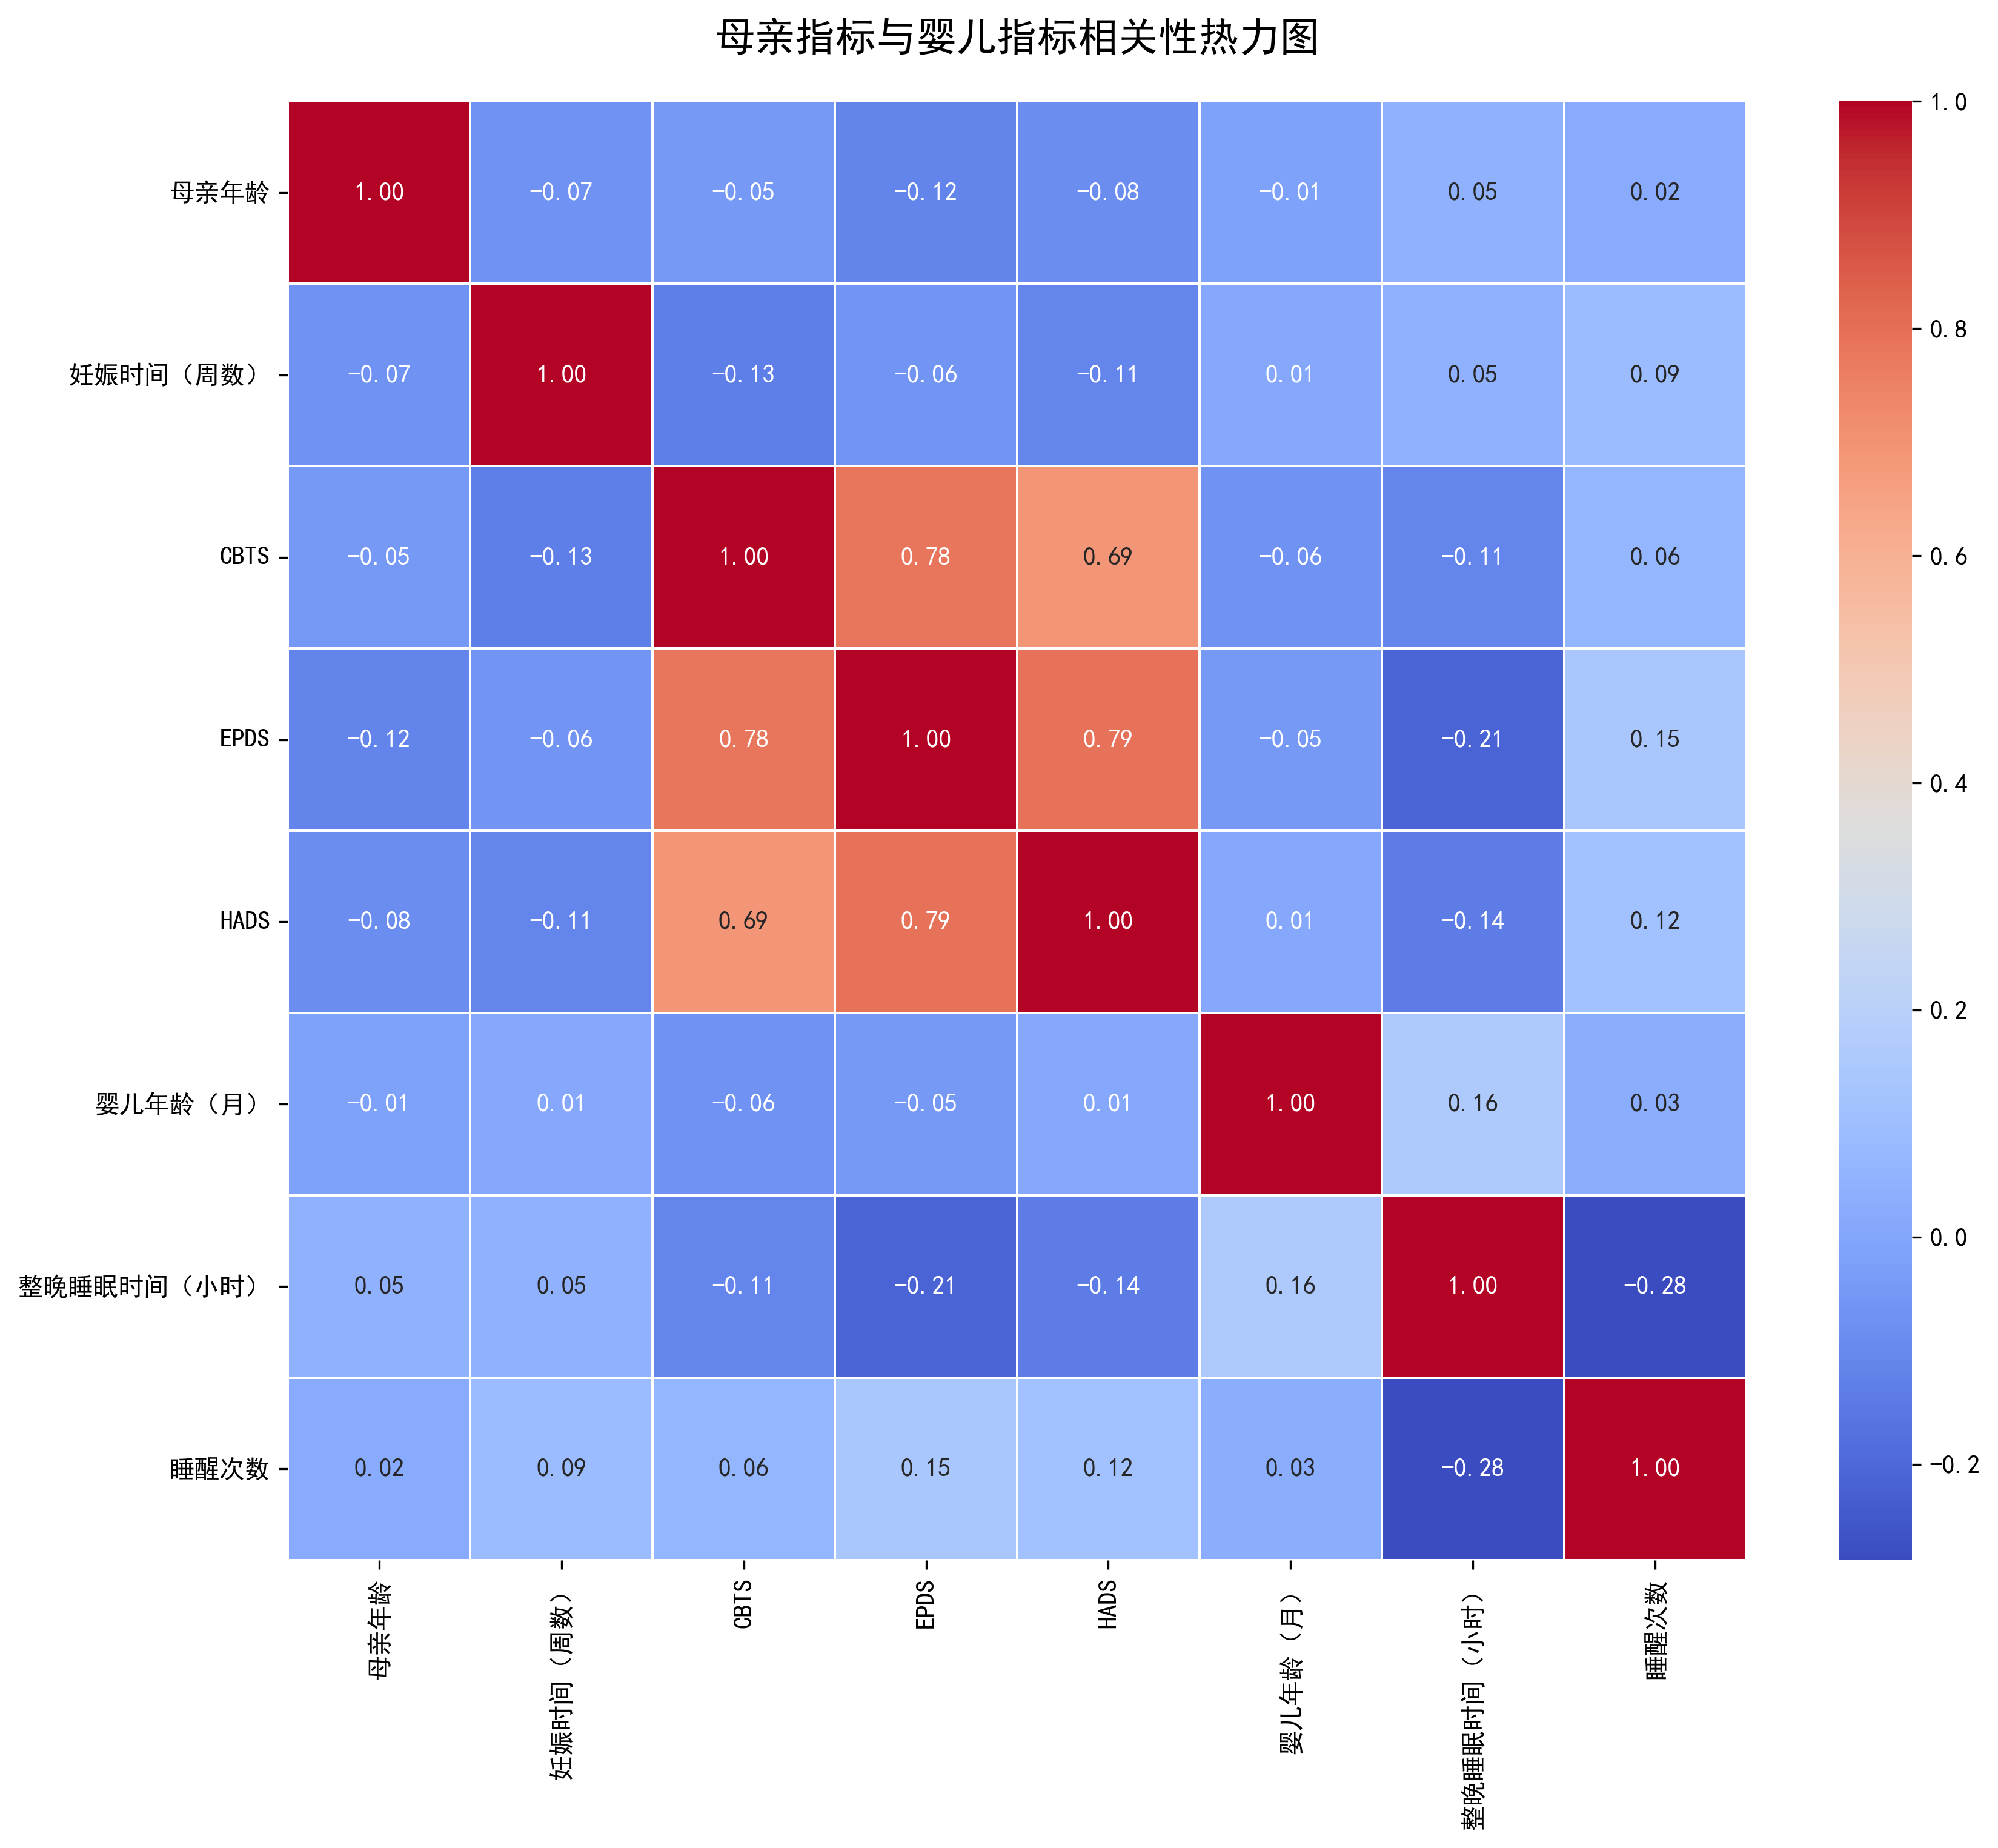
\includegraphics[width=0.8\textwidth]{figures/correlation_heatmap.png}
    \caption{母亲指标与婴儿指标相关性热力图}
    \label{fig:correlation_heatmap}
\end{figure}

\subsubsection{分类变量对连续变量的影响 (ANOVA)}
我们使用方差分析(ANOVA)检验了各分类变量对婴儿睡眠质量指标(睡醒次数、整晚睡眠时间)的影响。相关结果分别展示在图\ref{fig:anova_wake_up_times}和图\ref{fig:anova_sleep_time}中。
\begin{itemize}
    \item \textbf{入睡方式的显著影响}:
    \begin{itemize}
        \item 对睡醒次数:入睡方式对睡醒次数有显著影响($F=16.87, p<0.001$)。自主入睡的婴儿睡醒次数明显少于其他入睡方式。
        \item 对整晚睡眠时间:入睡方式对整晚睡眠时间也有显著影响($F=12.18, p<0.001$)。自主入睡的婴儿整晚睡眠时间明显长于其他入睡方式。
    \end{itemize}
    \item \textbf{其他分类变量影响不显著}:婚姻状况、教育程度、分娩方式、婴儿性别对睡眠质量的影响均不显著($p>0.05$)。
\end{itemize}

\begin{figure}[htbp]
    \centering
    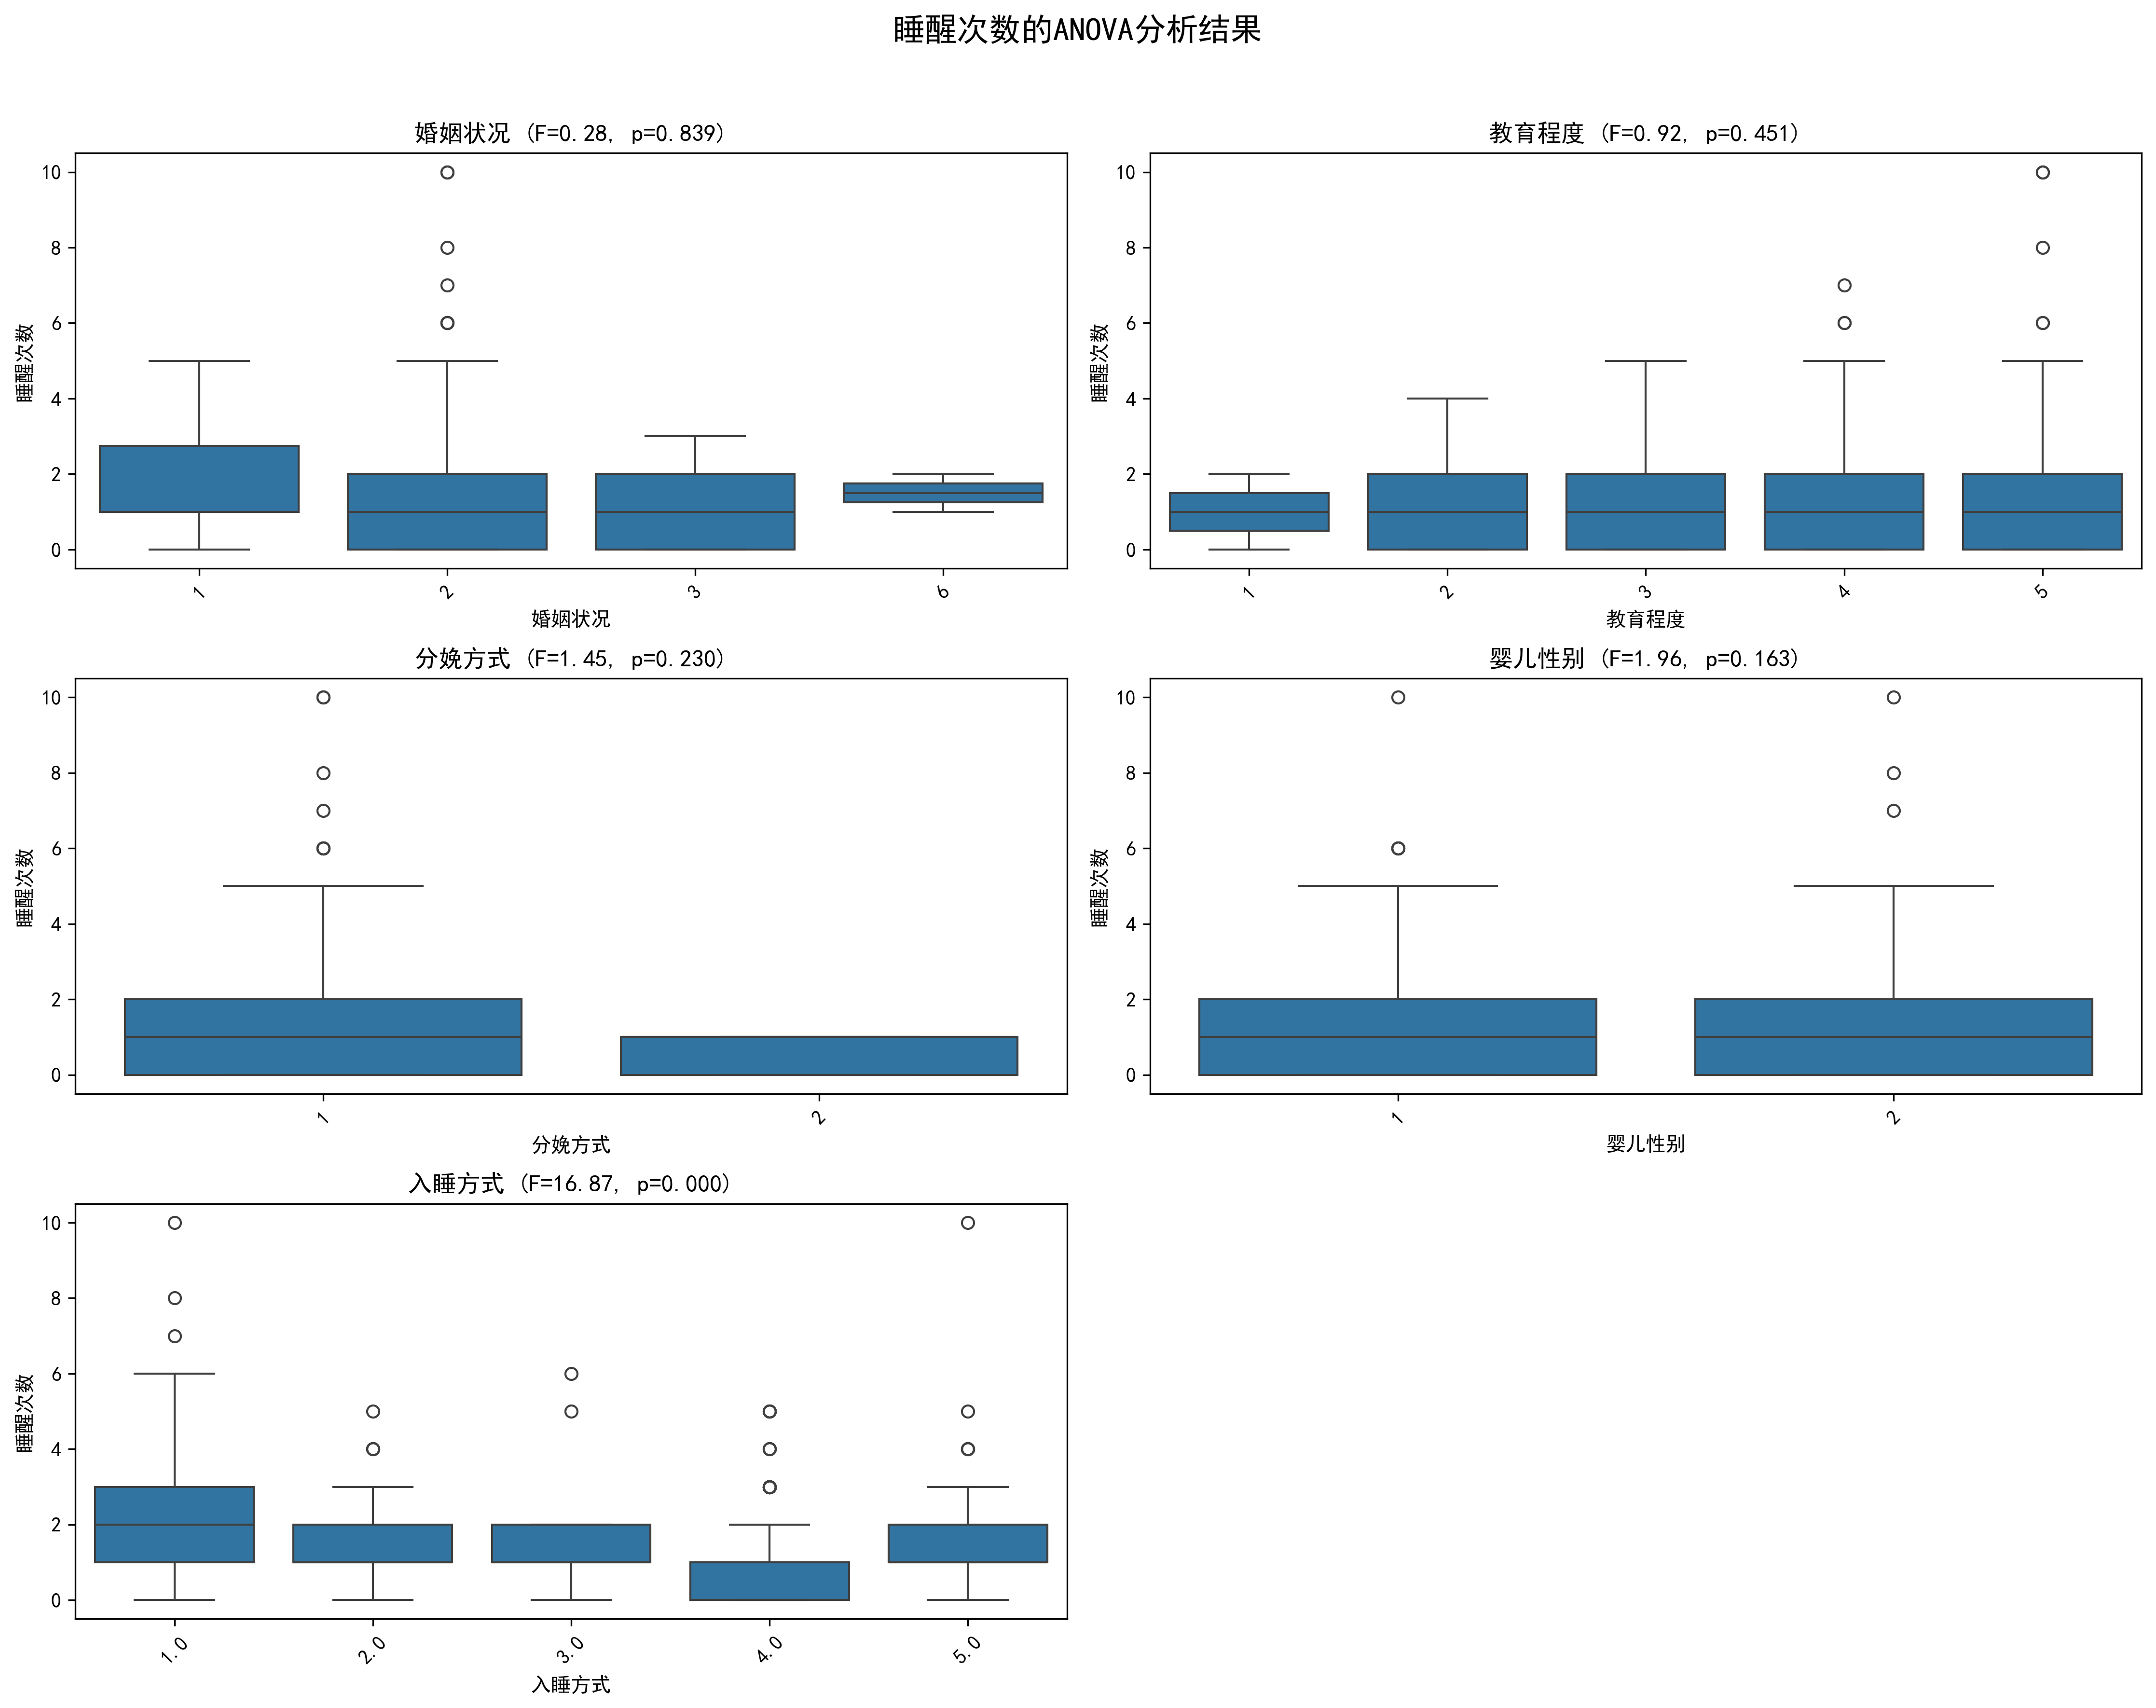
\includegraphics[width=0.9\textwidth]{figures/anova_睡醒次数_combined.png}
    \caption{睡醒次数的ANOVA分析结果}
    \label{fig:anova_wake_up_times}
\end{figure}

\begin{figure}[htbp]
    \centering
    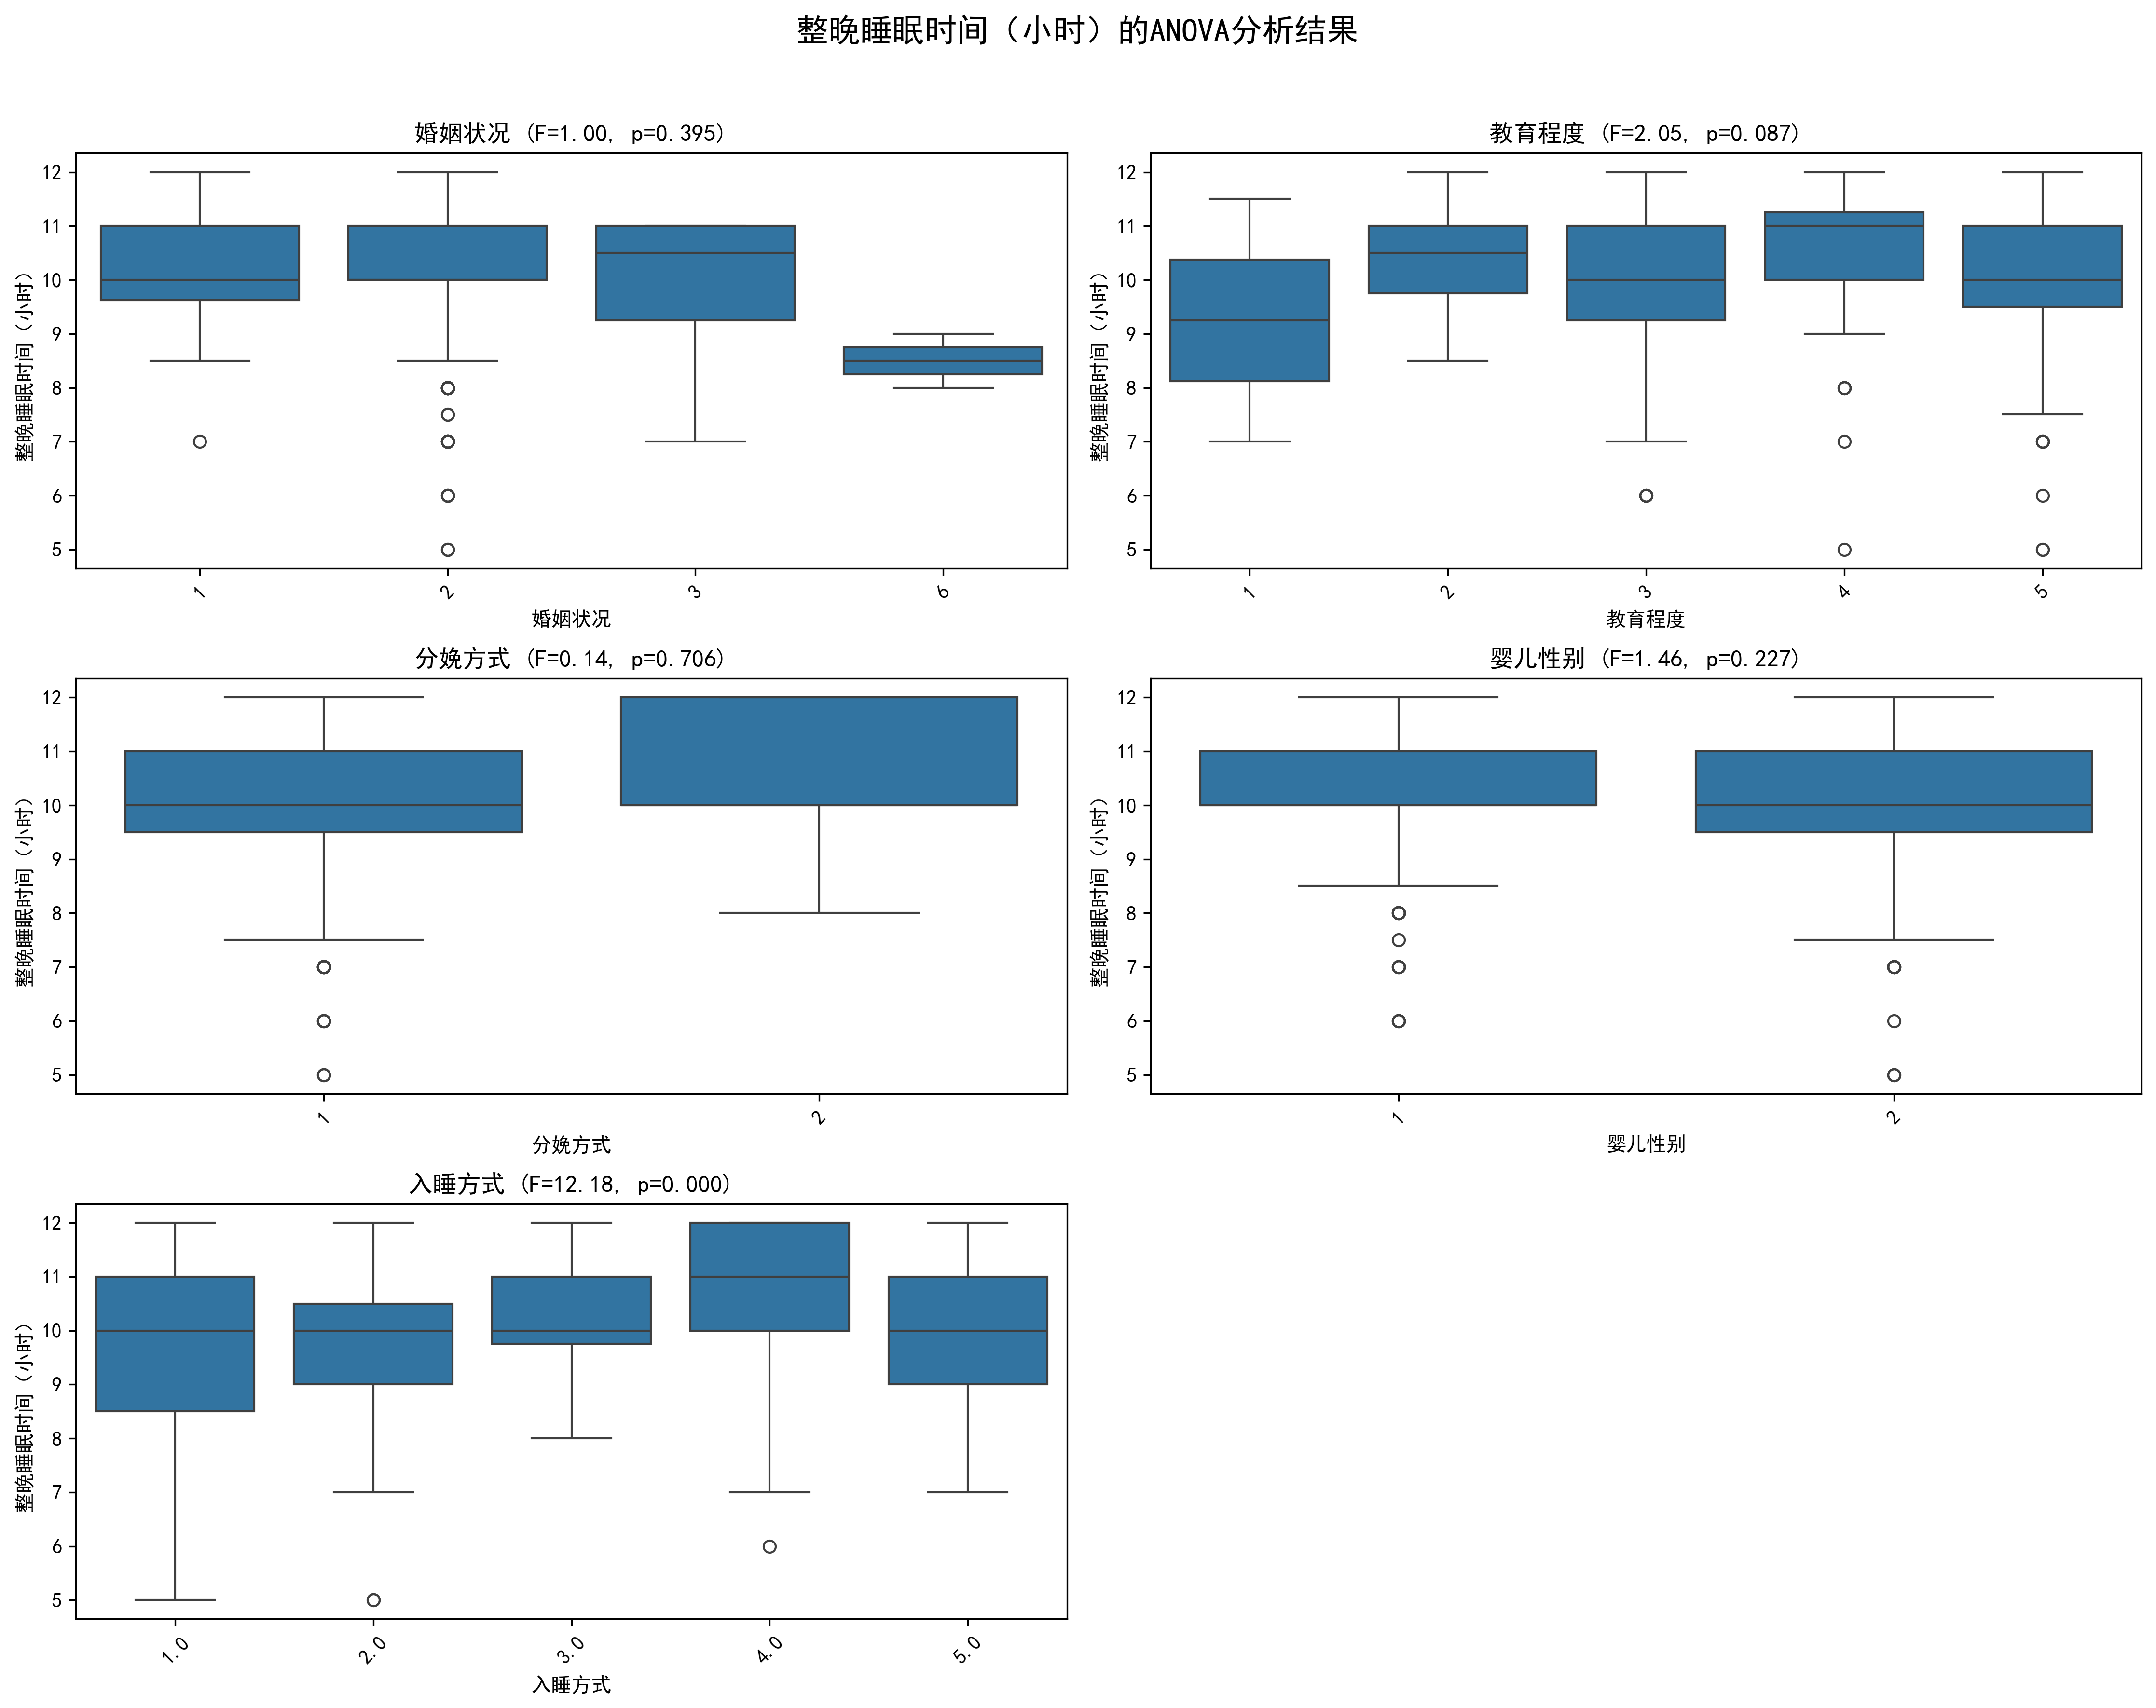
\includegraphics[width=0.9\textwidth]{figures/anova_整晚睡眠时间(小时)_combined.png}
    \caption{整晚睡眠时间(小时)的ANOVA分析结果}
    \label{fig:anova_sleep_time}
\end{figure}

\subsubsection{分类变量间的关联性 (Chi-square)}
我们利用卡方检验(Chi-square test)评估了分类变量之间的关联性。图\ref{fig:chi_square_significant}展示了具有统计显著性($p<0.05$)的分类变量对,而图\ref{fig:chi_square_p_values_heatmap}则以热力图形式呈现了所有分类变量对的p值。
\begin{itemize}
    \item \textbf{婚姻状况与教育程度的关联}:婚姻状况与教育程度之间存在显著关联($p=0.020$),表明已婚母亲的教育程度普遍较高。
    \item \textbf{入睡方式与婴儿行为特征的关联}:入睡方式与婴儿行为特征之间存在显著关联($p=0.014$),自主入睡的婴儿更倾向于安静型行为特征。
    \item 大多数分类变量之间没有显著关联,表明这些因素相对独立。
\end{itemize}

\begin{figure}[htbp]
    \centering
    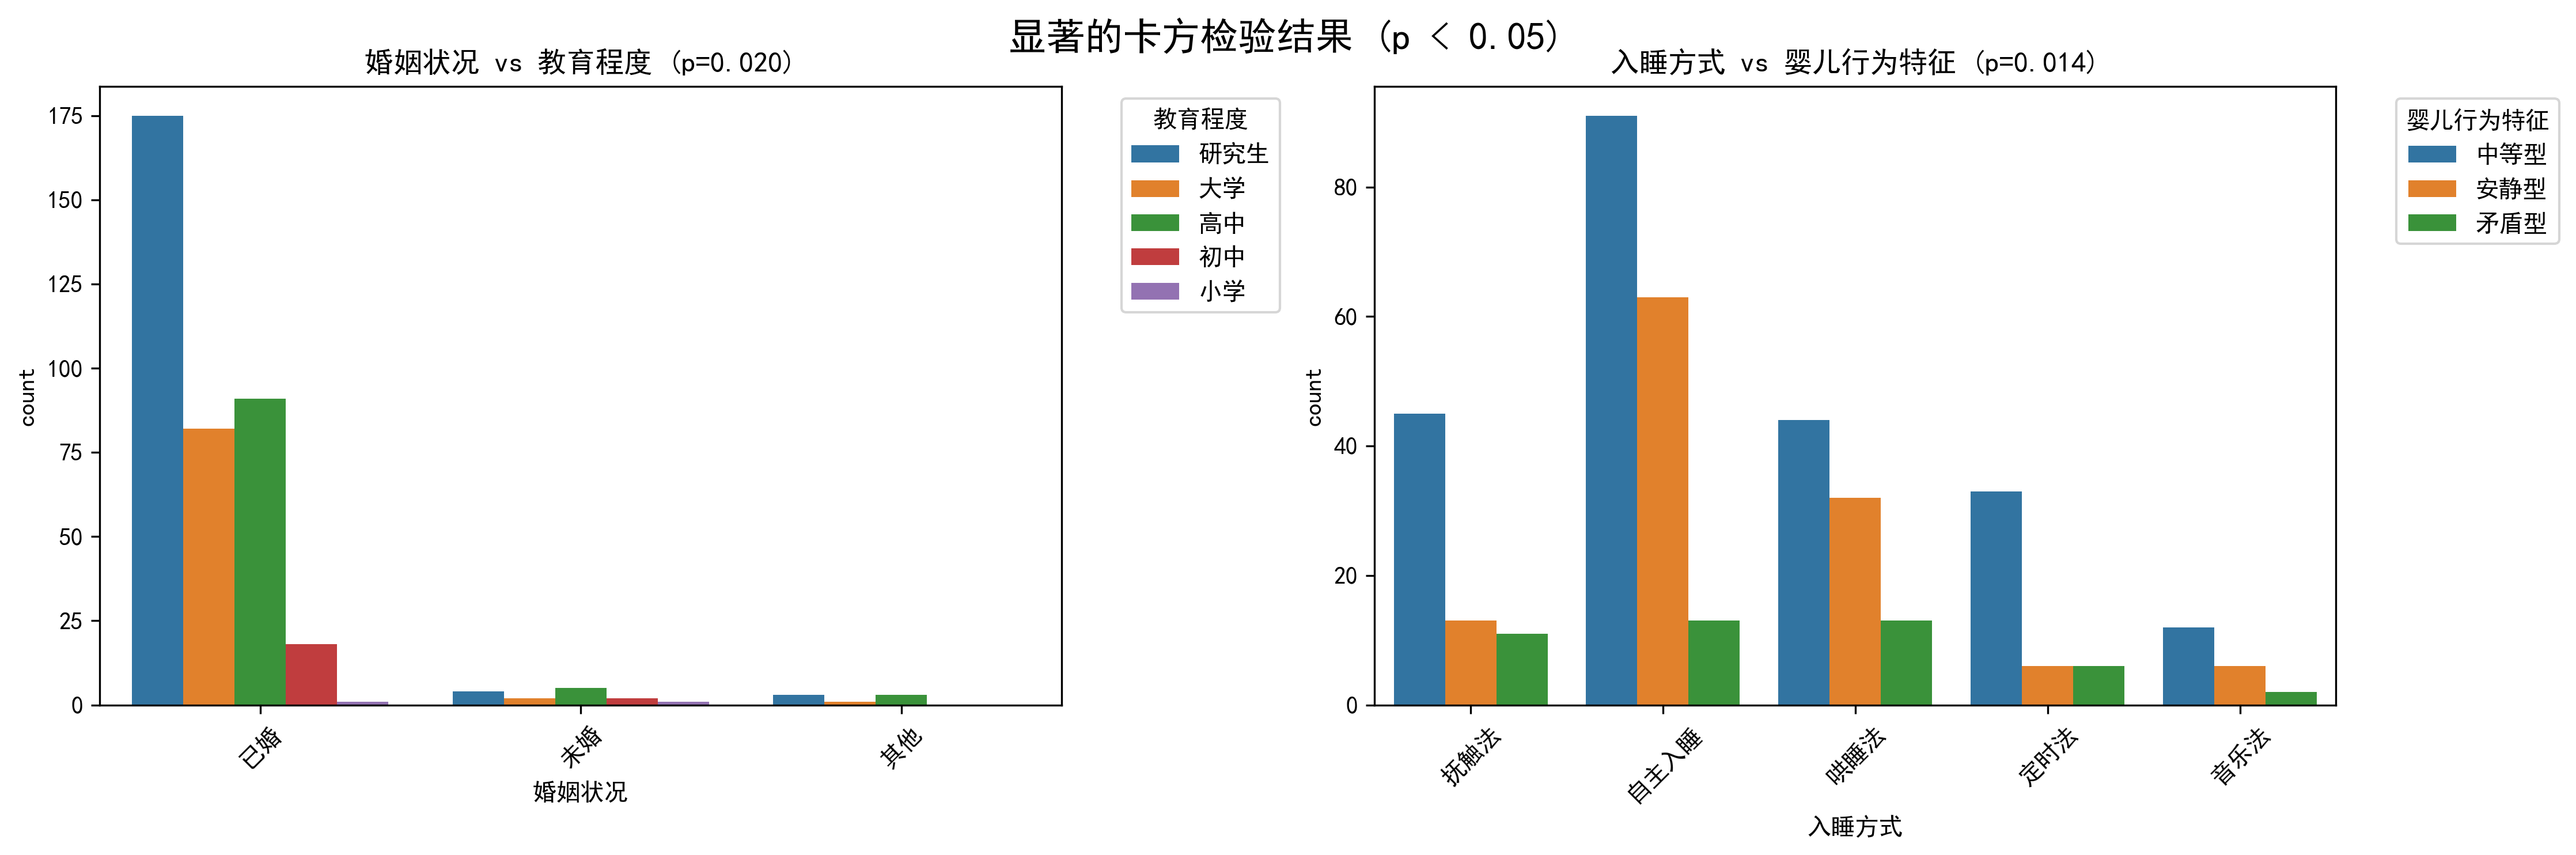
\includegraphics[width=0.9\textwidth]{figures/chi_square_significant_results.png}
    \caption{显著的卡方检验结果 ($p < 0.05$)}
    \label{fig:chi_square_significant}
\end{figure}

\begin{figure}[htbp]
    \centering
    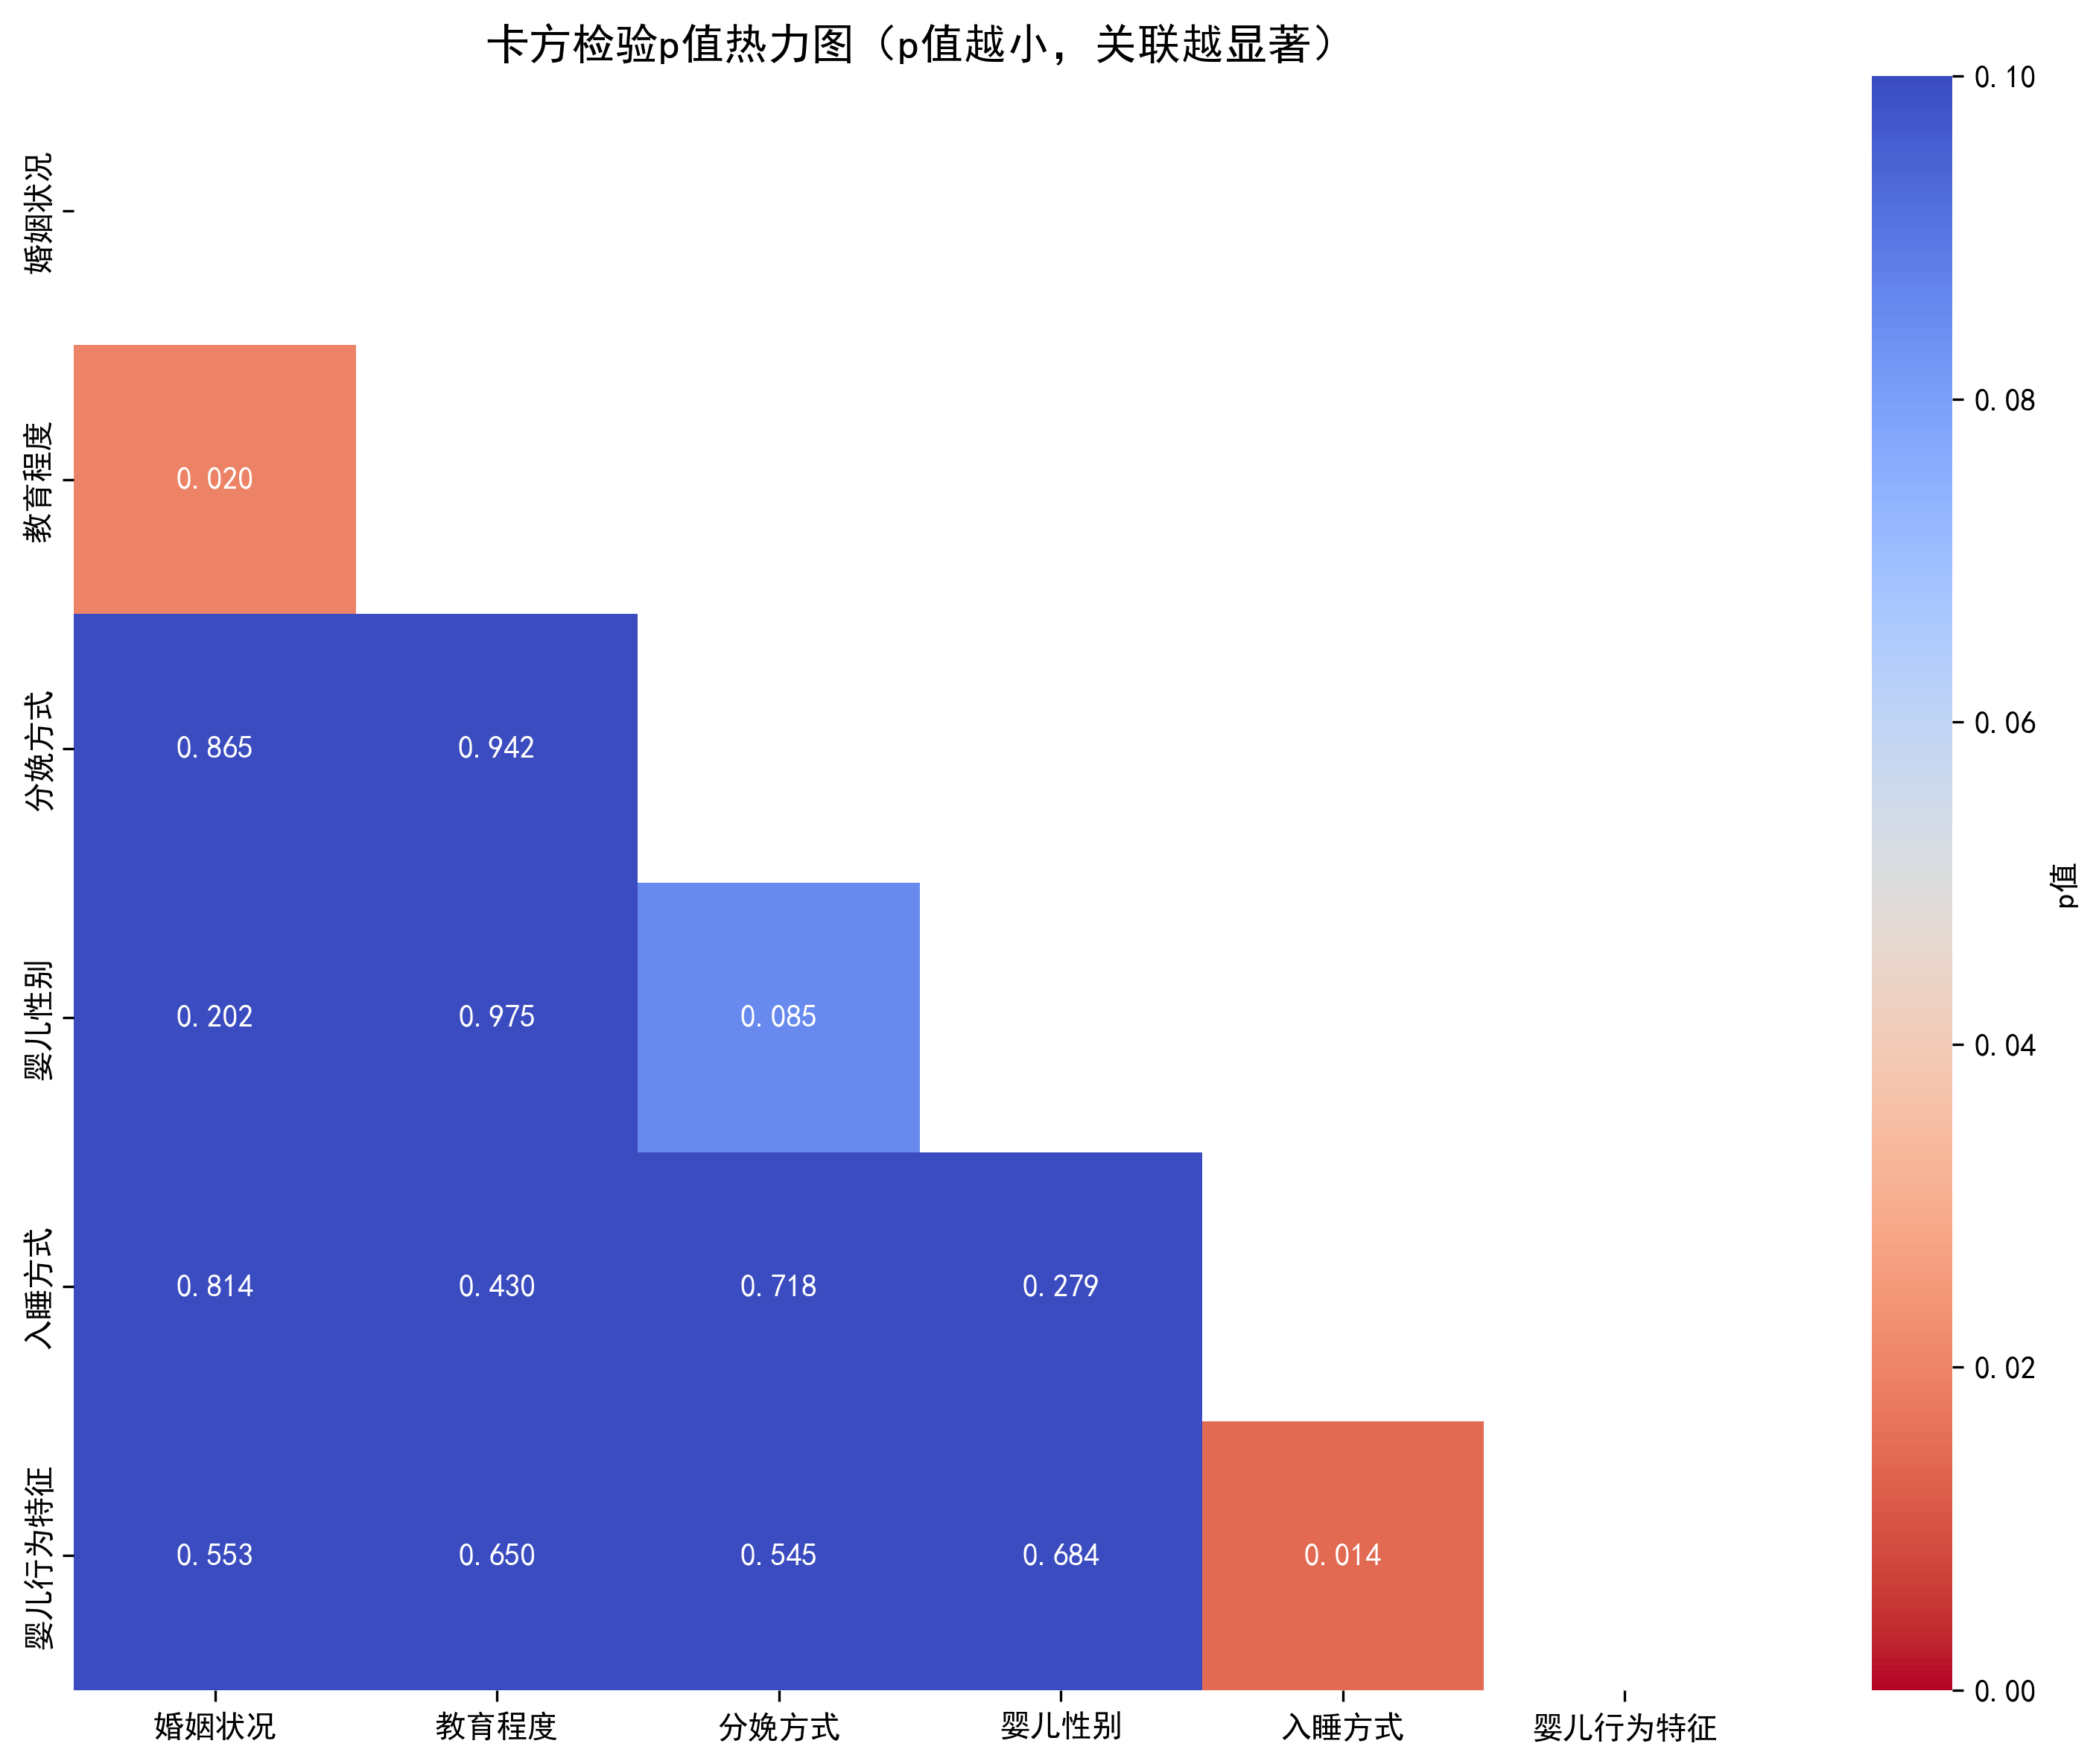
\includegraphics[width=0.6\textwidth]{figures/chi_square_p_values_heatmap.png}
    \caption{卡方检验p值热力图 (p值越小,关联越显著)}
    \label{fig:chi_square_p_values_heatmap}
\end{figure}

\subsubsection{多重共线性检查}
为了评估模型中自变量之间的多重共线性问题,我们计算了各预测变量的方差膨胀因子(VIF)。如图\ref{fig:multicollinearity_vif}所示:
\begin{itemize}
    \item 教育程度\_研究生的VIF值最高(5.72),接近但未超过常用的警戒线(VIF=10),表明存在一定的共线性但仍在可接受范围。
    \item 教育程度\_高中和教育程度\_大学的VIF值也较高(分别为4.56和4.36)。
    \item EPDS的VIF值为3.94,反映了与其他心理指标之间存在一定相关性。
    \item 大多数变量的VIF值小于2.5,表明多重共线性问题总体可控,不会严重影响模型结果的稳定性或解释力。
\end{itemize}

\begin{figure}[htbp]
    \centering
    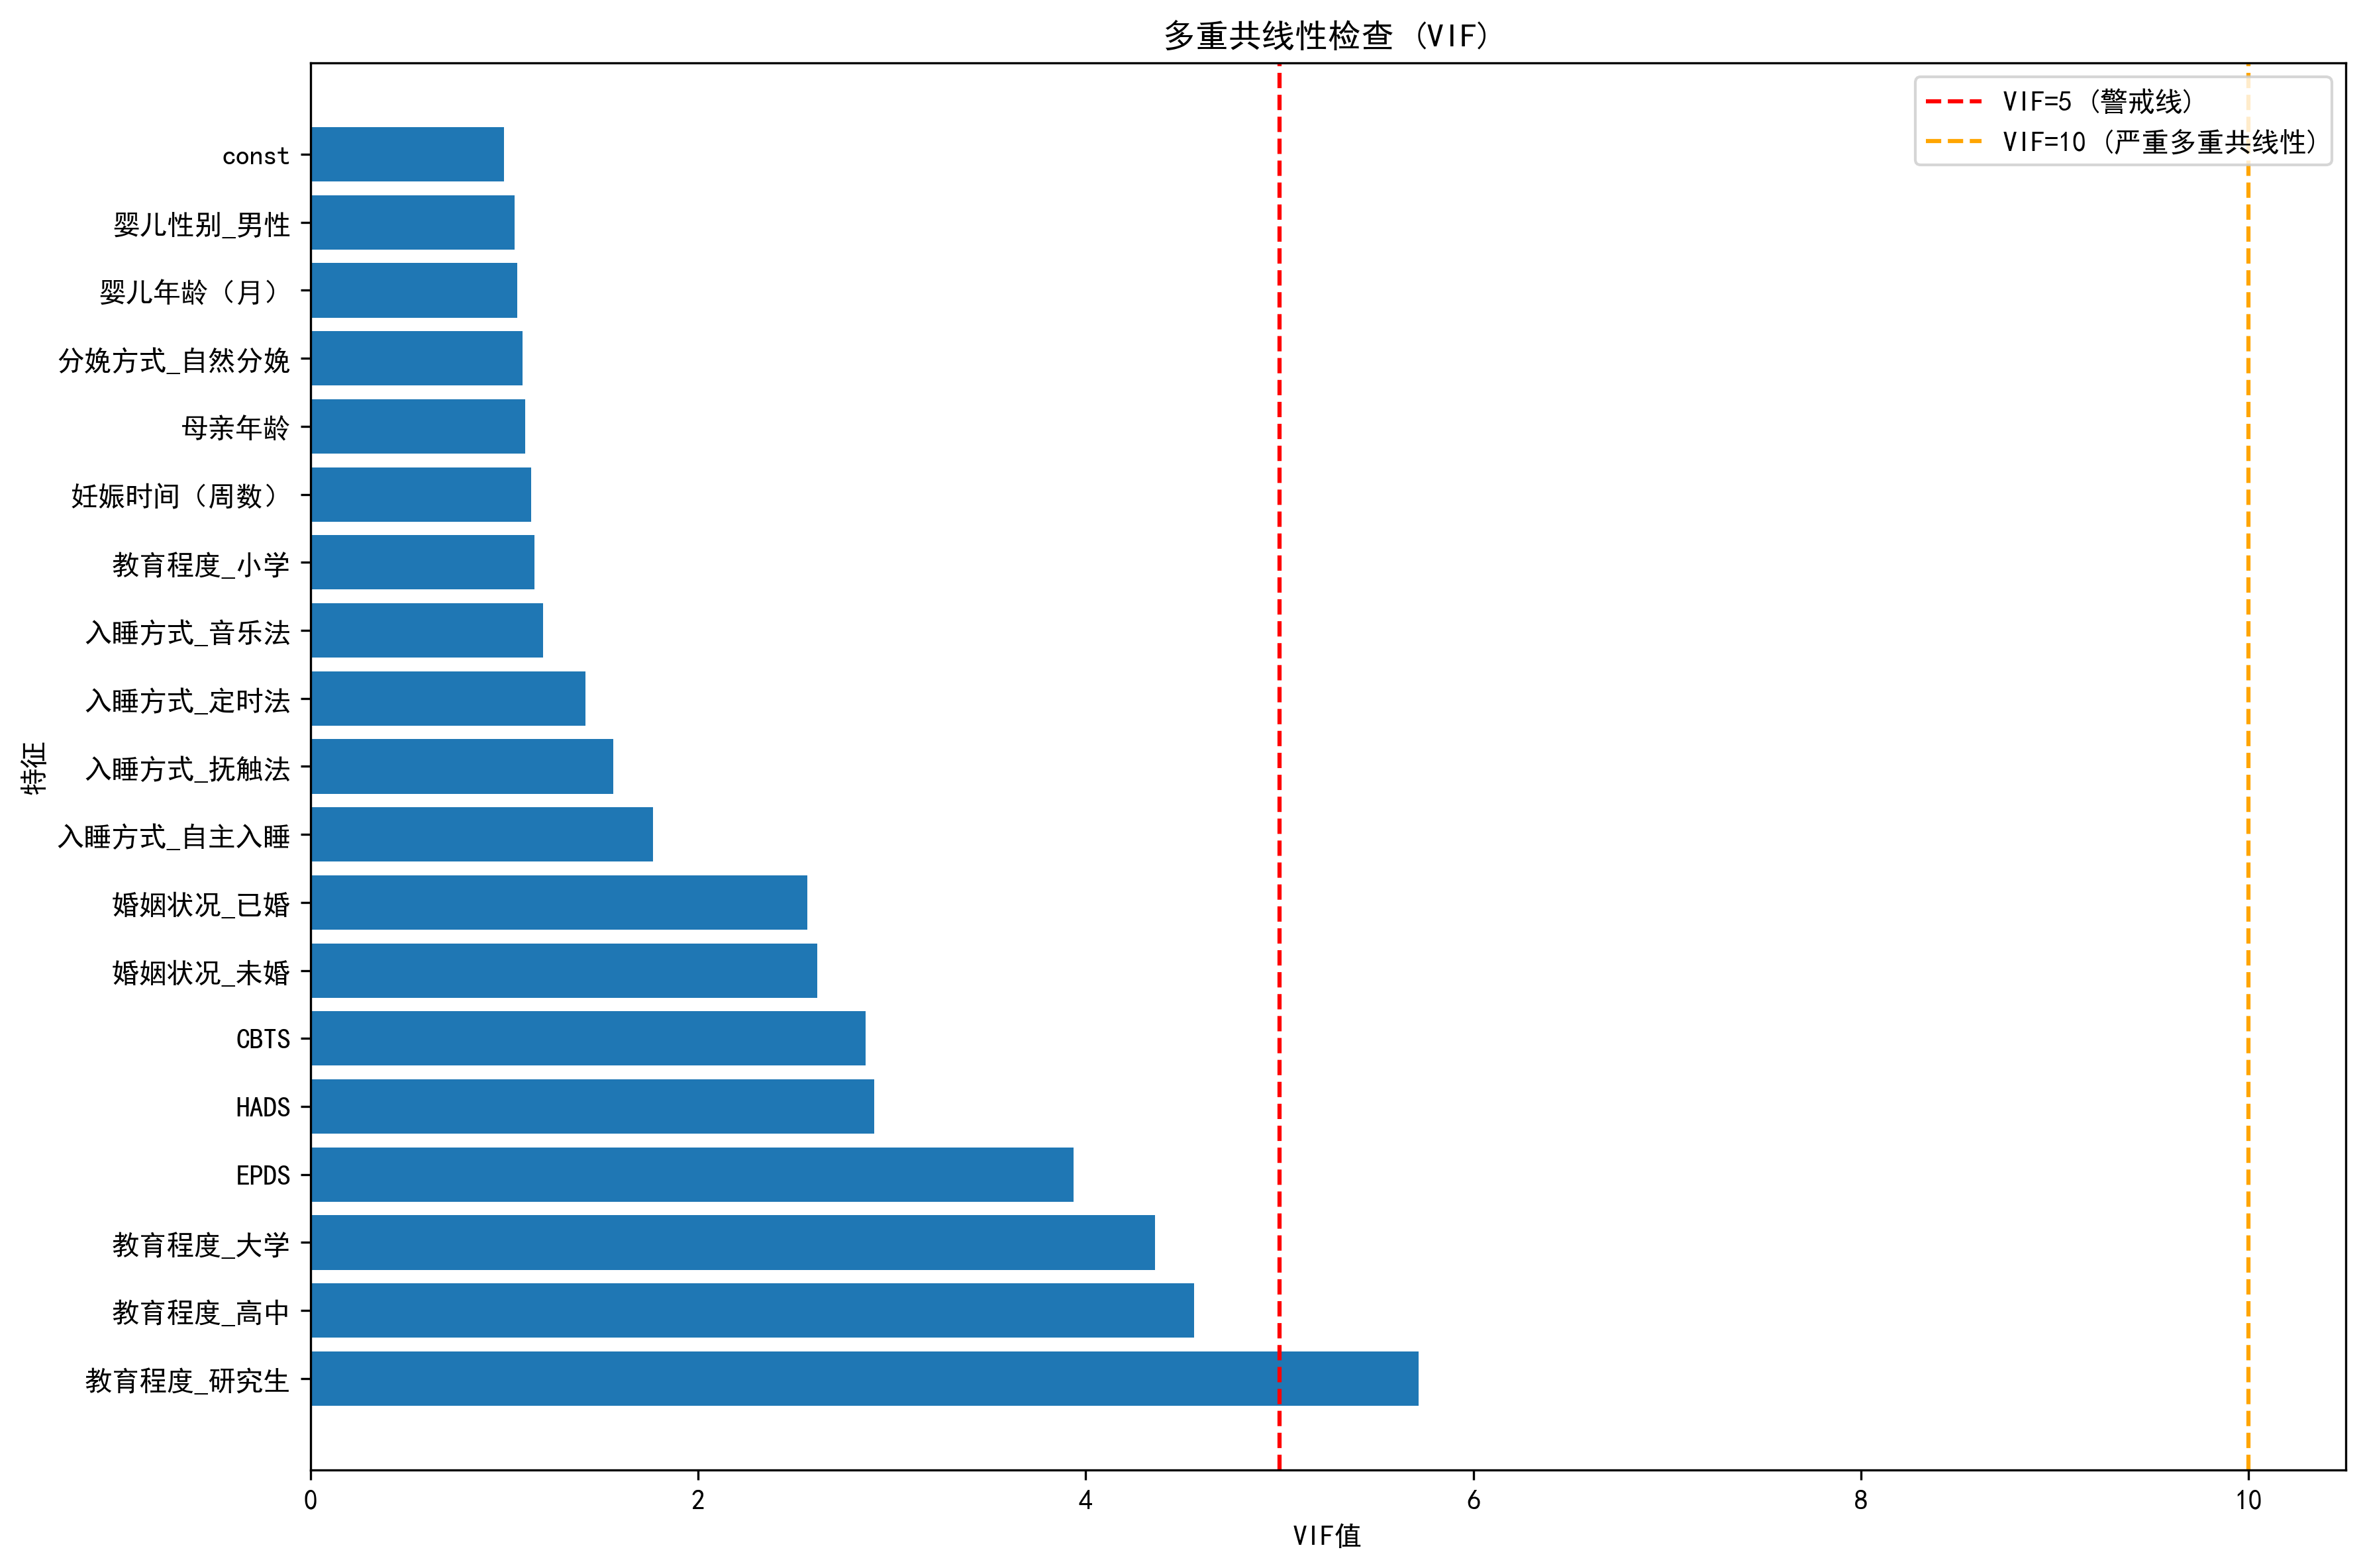
\includegraphics[width=0.7\textwidth]{figures/multicollinearity_vif.png}
    \caption{多重共线性检查 (VIF)}
    \label{fig:multicollinearity_vif}
\end{figure}

\subsection{模型选择与理论基础}
根据问题一所涉因变量的类型(连续型与多分类型),我们选择了相应的统计回归模型进行分析。

\subsubsection{婴儿睡眠质量模型:多元线性回归}
由于婴儿的“整晚睡眠时间”和“睡醒次数”均为连续数值型变量,我们选择多元线性回归 (Multiple Linear Regression) 作为其预测模型。多元线性回归旨在建立一个线性关系,用一个或多个自变量来预测因变量的取值。
其一般形式为:
$$ Y = \beta_0 + \beta_1 X_1 + \beta_2 X_2 + \dots + \beta_k X_k + \epsilon $$
其中:
\begin{itemize}
    \item $Y$ 是因变量(如整晚睡眠时间或睡醒次数)。
    \item $X_1, X_2, \dots, X_k$ 是 $k$ 个自变量(如母亲年龄、心理指标、入睡方式等)。
    \item $\beta_0$ 是截距项。
    \item $\beta_1, \beta_2, \dots, \beta_k$ 是对应自变量的回归系数,表示在其他自变量不变的情况下,该自变量每增加一个单位,因变量的平均变化量。
    \item $\epsilon$ 是误差项,代表模型未能解释的随机变异。
\end{itemize}
模型通过最小化残差平方和(Ordinary Least Squares, OLS)来估计回归系数。模型的评估指标包括决定系数 ($R^2$)、调整决定系数 (Adjusted $R^2$)、F统计量及其p值,用于评估模型的整体拟合优度和统计显著性。

\subsubsection{婴儿行为特征模型:多项逻辑回归}
婴儿行为特征(“安静型”、“中等型”、“矛盾型”)是一个具有三个或更多无序类别的分类变量。因此,我们选择多项逻辑回归 (Multinomial Logistic Regression) 模型来分析母亲各项因素对其影响。多项逻辑回归是二元逻辑回归的扩展,用于预测一个多分类因变量的概率。
它通过建立多个二元逻辑回归模型来比较每个类别与一个基准类别(参考类别)的对数发生比 (log-odds)。假设我们有 $J$ 个类别,选择第 $J$ 个类别作为参考类别。对于每个非参考类别 $j \in \{1, \dots, J-1\}$,模型估计其相对于参考类别的对数发生比:
$$ \ln\left(\frac{P(Y=j | \mathbf{X})}{P(Y=J | \mathbf{X})}\right) = \beta_{j0} + \beta_{j1} X_1 + \beta_{j2} X_2 + \dots + \beta_{jk} X_k $$
其中:
\begin{itemize}
    \item $P(Y=j | \mathbf{X})$ 是在给定自变量 $\mathbf{X}$ 的情况下,因变量属于类别 $j$ 的概率。
    \item $\beta_{j}$ 是对应于类别 $j$ 的回归系数向量。
\item 发生比 (Odds Ratio, OR):$e^{\beta_{ji}}$ 表示在其他自变量不变的情况下,自变量 $X_i$ 每增加一个单位,因变量属于类别 $j$ 而而非参考类别的发生比的变化倍数。
\end{itemize}
模型的评估通常使用赤池信息准则 (AIC) 和贝叶斯信息准则 (BIC),它们平衡了模型的拟合优度和复杂度。发生比 (Odds Ratio) 的可视化是理解自变量对不同类别影响的关键。

\subsection{模型构建与求解}
在确定模型类型后,我们基于前期探索性数据分析的结果,构建并求解了各个模型。

\subsubsection{婴儿睡眠质量线性回归模型构建}
我们分别构建了预测“整晚睡眠时间”和“睡醒次数”的线性回归模型。模型纳入了所有经过预处理的母亲身体指标、心理指标以及独热编码后的分类变量。

\paragraph{整晚睡眠时间模型}
模型整体显著 ($F=4.66, p < 0.001$),但解释力有限 ($R^2 = 0.184$, Adjusted $R^2 = 0.145$)。这表明模型捕捉到了一部分变异,但婴儿睡眠时间受多种复杂因素影响,现有变量仅解释了约18.4\%的变异。
\begin{itemize}
    \item \textbf{显著预测因子}:
    \begin{itemize}
        \item \textbf{入睡方式\_自主入睡}:自主入睡的婴儿整晚睡眠时间显著更长。这证实了前期ANOVA分析的发现,并强调了这一因素对婴儿睡眠质量的决定性作用。
        \item \textbf{EPDS得分}:母亲EPDS(爱丁堡产后抑郁量表)得分越高,婴儿整晚睡眠时间越短,呈现显著负相关。这揭示了母亲抑郁情绪对婴儿睡眠的负面影响。
    \end{itemize}
\end{itemize}

\paragraph{睡醒次数模型}
模型整体显著 ($F=5.32, p < 0.001$),解释力略高于睡眠时间模型 ($R^2 = 0.205$, Adjusted $R^2 = 0.167$)。
\begin{itemize}
    \item \textbf{显著预测因子}:
    \begin{itemize}
        \item \textbf{入睡方式}:入睡方式是影响睡醒次数的最显著因素。具体而言,自主入睡的婴儿睡醒次数明显更少。
        \item \textbf{HADS得分}:母亲HADS(医院焦虑抑郁量表)得分越高,婴儿睡醒次数越多,呈现显著正相关。这进一步印证了母亲心理健康状况与婴儿睡眠质量的紧密联系。
    \end{itemize}
\end{itemize}

\subsubsection{婴儿行为特征多项逻辑回归模型构建}
我们构建了多项逻辑回归模型来预测婴儿的行为特征。在此模型中,我们将“中等型”婴儿作为参考类别,分析其他两类(“安静型”和“矛盾型”)相对于“中等型”的发生比。
模型评估指标为 $AIC = 693.31$ 和 $BIC = 844.02$。虽然模型能够区分不同行为特征类型,但预测准确率仍有提升空间。图\ref{fig:baby_behavior_odds_ratios}展示了各变量对婴儿行为特征影响的发生比。
\begin{itemize}
    \item \textbf{显著预测因子与发生比分析}:
    \begin{itemize}
        \item \textbf{母亲心理指标 (CBTS, EPDS, HADS)}:这三项指标对婴儿行为特征有显著影响。母亲心理压力越大(即CBTS、EPDS、HADS得分越高),婴儿表现为“矛盾型”行为特征的可能性相对于“中等型”越大。这提示母亲心理健康问题可能导致婴儿出现更具挑战性的行为模式。
        \item \textbf{入睡方式}:入睡方式对婴儿行为特征具有显著影响。具体而言,与“中等型”婴儿相比,采用“自主入睡”方式的婴儿更倾向于表现为“安静型”行为特征。这再次强调了培养良好入睡习惯的重要性。
        \item \textbf{母亲教育程度}:母亲教育程度对婴儿行为特征也有一定影响。通常,教育程度越高的母亲,其婴儿表现为“安静型”的可能性越大。这可能反映了高教育程度母亲在育儿理念、环境创设或早期干预方面的优势。
    \end{itemize}
\end{itemize}

\begin{figure}[htbp]
    \centering
    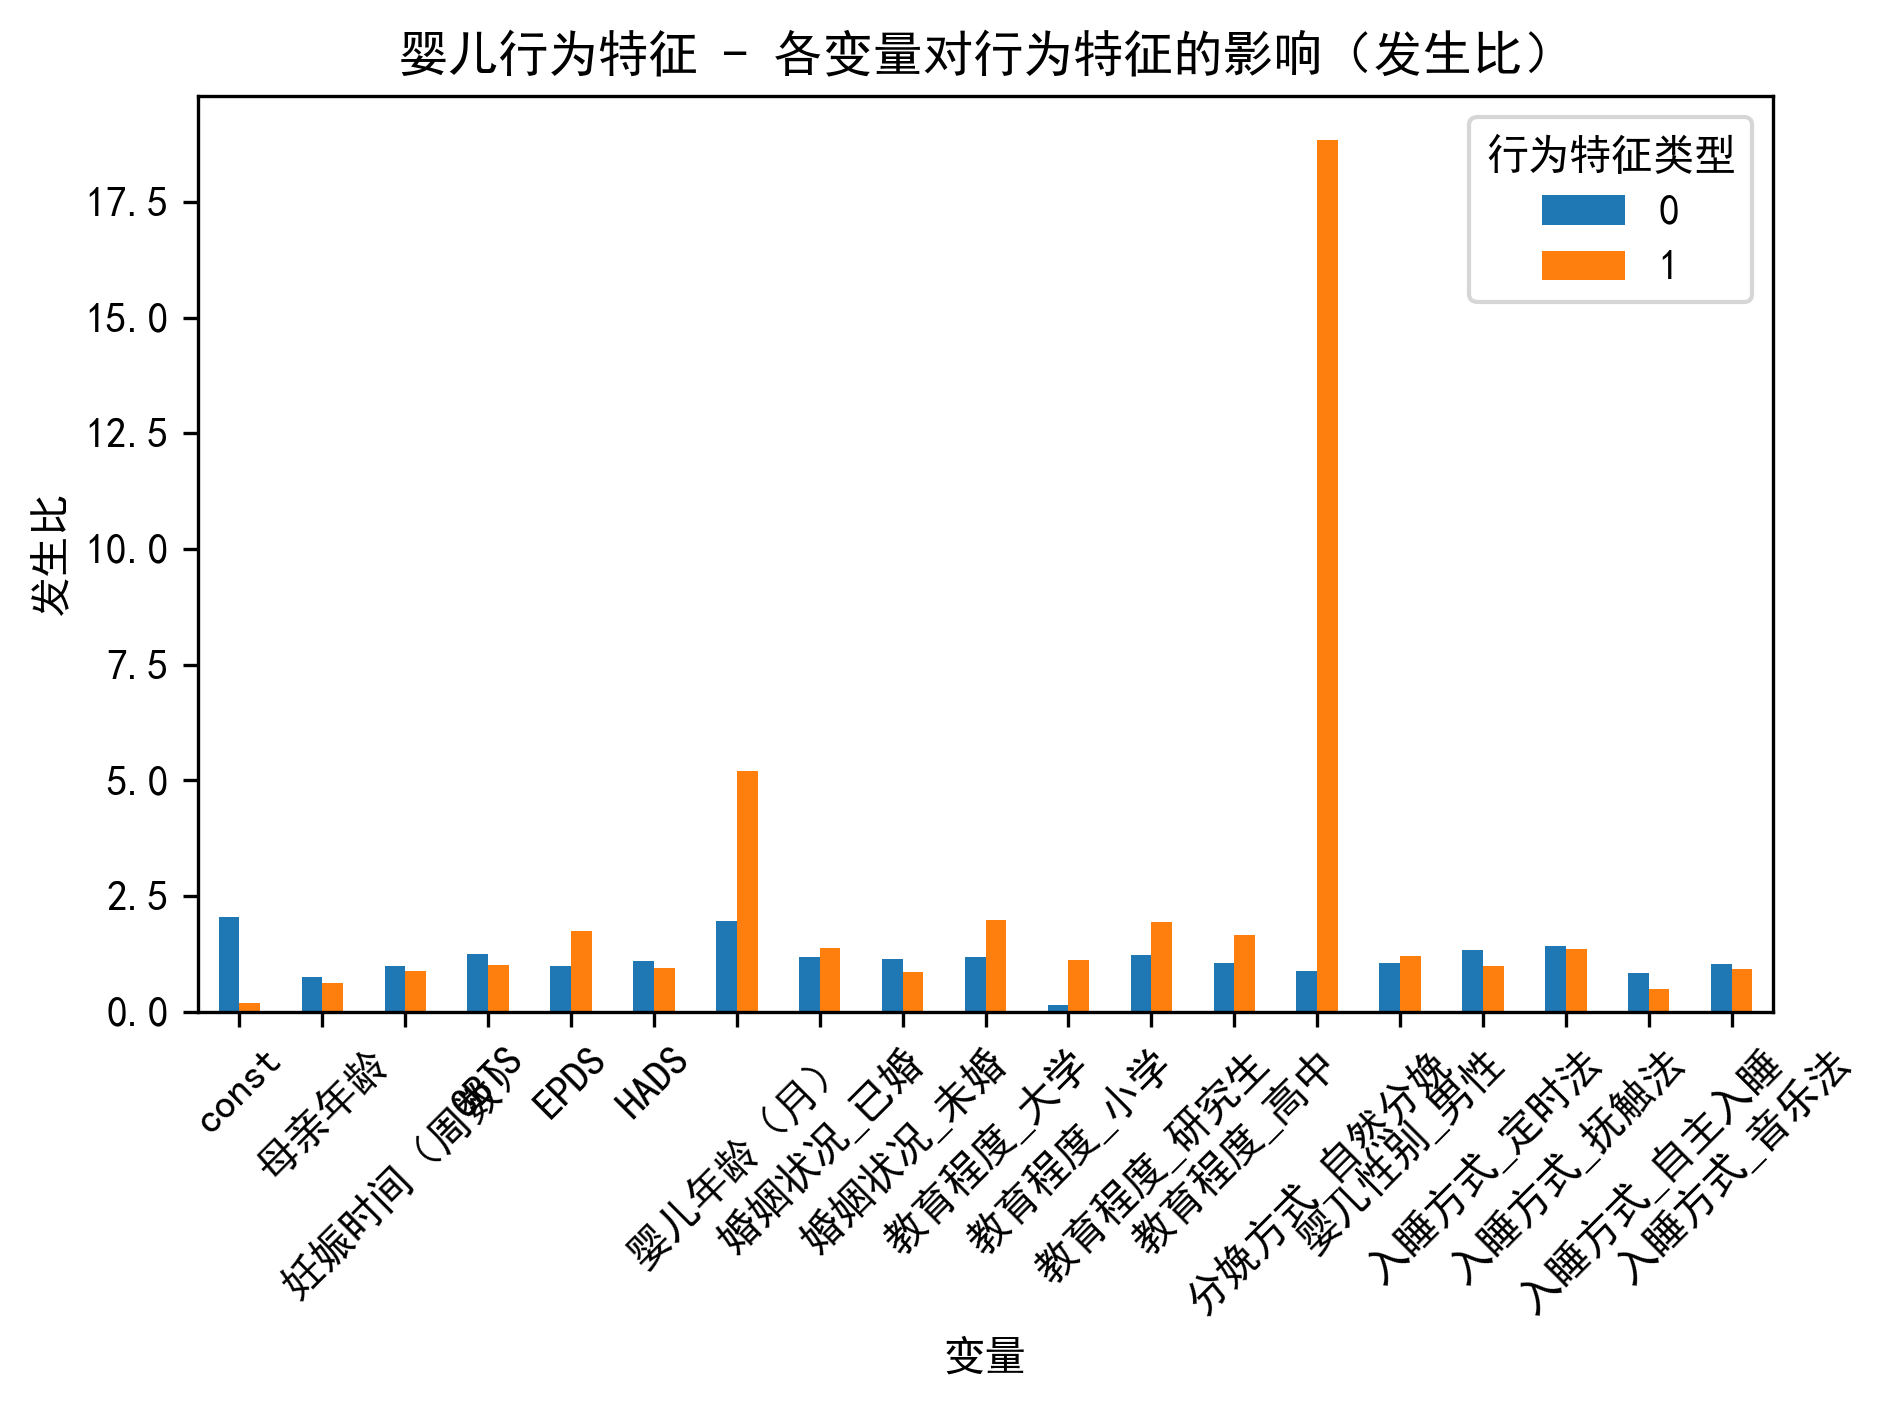
\includegraphics[width=0.8\textwidth]{figures/婴儿行为特征_odds_ratios.png} % 假设此图片文件也可用
    \caption{婴儿行为特征发生比可视化}
    \label{fig:baby_behavior_odds_ratios}
\end{figure}

\subsection{模型结果与分析}
综合上述线性回归与多项逻辑回归模型的结果,我们可以得出以下关键发现:

\begin{enumerate}
    \item \textbf{母亲心理健康是婴儿发展的重要决定因素}:
    我们的模型一致表明,母亲的抑郁(EPDS)、焦虑(HADS)和分娩相关创伤后应激(CBTS)症状与婴儿的睡眠质量和行为特征之间存在显著关联。具体表现为:母亲的心理压力越大,婴儿的整晚睡眠时间越短,睡醒次数越多,且更倾向于表现出“矛盾型”行为特征。这一发现强调了在产妇保健中纳入心理健康筛查与干预的重要性。
    \item \textbf{入睡方式对婴儿睡眠与行为具有核心影响}:
    无论是整晚睡眠时间、睡醒次数,还是婴儿行为特征,入睡方式均被识别为最关键的影响因素之一。自主入睡的婴儿普遍拥有更长的整晚睡眠时间,更少的睡醒次数,并且更可能表现为“安静型”行为。这为育儿实践提供了明确的指导:培养婴儿的自主入睡能力是改善其睡眠和行为的有效途径。
    \item \textbf{模型解释力与个体差异}:
    尽管模型整体具有统计显著性,但线性回归模型的 $R^2$ 值相对较低(约0.18-0.20),表明现有变量仅能解释婴儿睡眠质量变异的一小部分。这提示婴儿的睡眠和行为发展受到多方面因素的复杂影响,除了我们纳入的母亲身心健康和育儿方式外,可能还存在其他未被量化或收集的遗传、环境、生理等因素,从而导致显著的个体差异。因此,在实践中,干预措施需要考虑个体化和多维度支持。
    \item \textbf{心理指标的协同作用}:
    母亲的CBTS、EPDS和HADS之间存在高度相关性,提示这些心理困扰并非孤立存在,而是相互关联、可能同时出现的。在多项逻辑回归中,它们共同作用于婴儿行为特征。这提示在临床干预中,应采取综合性的心理支持策略,而非仅关注单一症状。
\end{enumerate}
这些模型分析结果为理解母亲身心健康与婴儿早期发展的复杂关系提供了量化证据,并为未来的干预策略指明了方向。尽管模型解释力存在局限性,但其识别的关键影响因素具有重要的实践指导意义。


%%%%%%%%%%%%%%%%%%%%%%%%%%%%%%%%%%%%%%%%%%%%%%%%%%%%%%%%%%%%% 

\section{问题二的模型的建立和求解}
\subsection{模型建立}

引用\cref{fig:双图},引用\cref{fig:双图a},引用\cref{fig:双图b}。

\begin{figure}[ht]
\centering
\subcaptionbox{双图a子标题\label{fig:双图a}}
{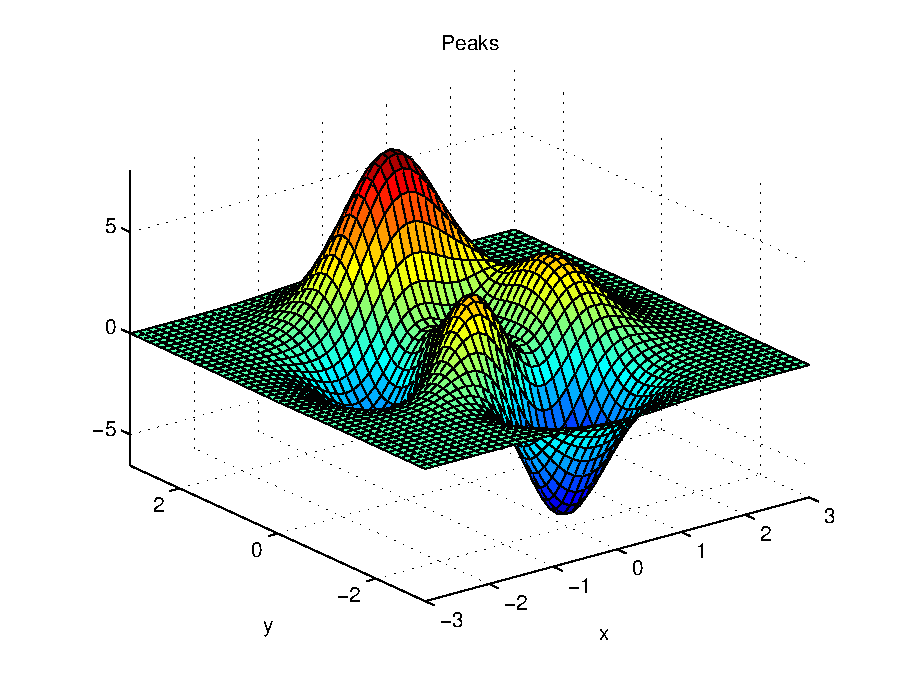
\includegraphics[width=.4\textwidth]{example.eps}}
\subcaptionbox{双图b子标题\label{fig:双图b}}
{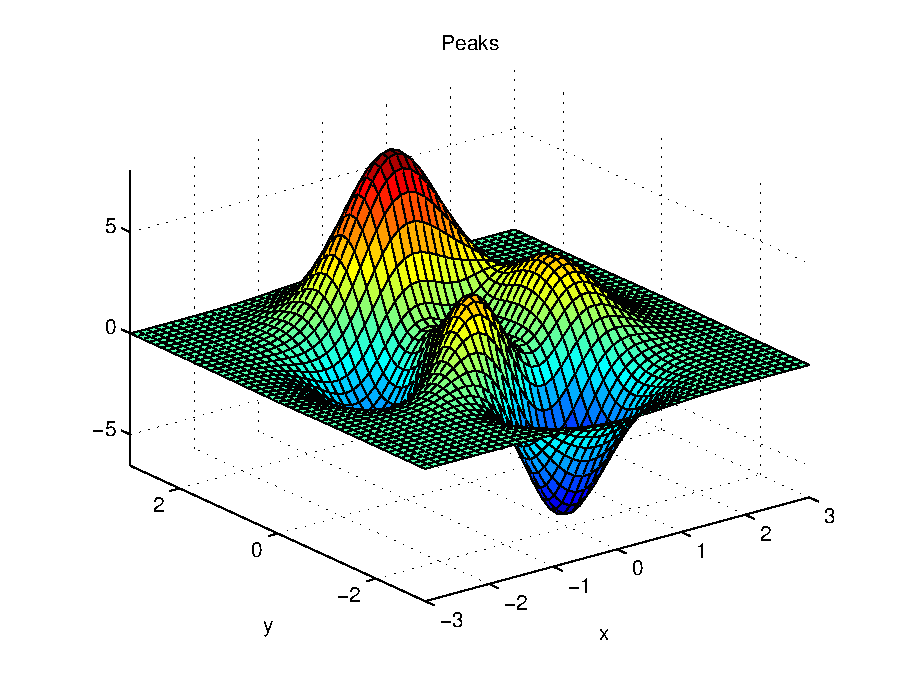
\includegraphics[width=.4\textwidth]{example.eps}}
\caption{双图}\label{fig:双图}
\end{figure} 

\subsection{模型求解}

\textbf{Step1:} 

\textbf{Step2:} 

\textbf{Step3:} 

\subsection{求解结果}

%%%%%%%%%%%%%%%%%%%%%%%%%%%%%%%%%%%%%%%%%%%%%%%%%%%%%%%%%%%%% 

\section{问题三的模型的建立和求解}
\subsection{模型建立}

\subsection{模型求解}

\textbf{Step1:} 

\textbf{Step2:} 

\textbf{Step3:} 

\subsection{求解结果}

%%%%%%%%%%%%%%%%%%%%%%%%%%%%%%%%%%%%%%%%%%%%%%%%%%%%%%%%%%%%% 

\section{问题四的模型的建立和求解}
\subsection{模型建立}

\subsection{模型求解}

\textbf{Step1:} 

\textbf{Step2:} 

\textbf{Step3:} 

\subsection{求解结果}

%%%%%%%%%%%%%%%%%%%%%%%%%%%%%%%%%%%%%%%%%%%%%%%%%%%%%%%%%%%%%

\section{模型的分析与检验}

\subsection{灵敏度分析}

\subsection{误差分析}

%%%%%%%%%%%%%%%%%%%%%%%%%%%%%%%%%%%%%%%%%%%%%%%%%%%%%%%%%%%%%

\section{模型的评价}

\subsection{模型的优点}
\begin{itemize}[itemindent=2em]
\item 优点1
\item 优点2
\item 优点3
\end{itemize}

\subsection{模型的缺点}
\begin{itemize}[itemindent=2em]
\item 缺点1
\item 缺点2
\end{itemize}

%%%%%%%%%%%%%%%%%%%%%%%%%%%%%%%%%%%%%%%%%%%%%%%%%%%%%%%%%%%%%
%% 参考文献
\nocite{*}
\bibliographystyle{gbt7714-numerical}  % 引用格式
\bibliography{ref.bib}  % bib源

\newpage
%%%%%%%%%%%%%%%%%%%%%%%%%%%%%%%%%%%%%%%%%%%%%%%%%%%%%%%%%%%%%
%% 附录
\begin{appendices}
\section{文件列表}
\begin{table}[H]
\centering
\begin{tabularx}{\textwidth}{LL}
\toprule
文件名   & 功能描述 \\
\midrule
q1.m & 问题一程序代码 \\
q2.py & 问题二程序代码 \\
q3.c & 问题三程序代码 \\
q4.cpp & 问题四程序代码 \\
\bottomrule
\end{tabularx}
\label{tab:文件列表}
\end{table}

\section{代码}
\noindent q1.m
\lstinputlisting[language=matlab]{code/q1.m}
q2.py
\lstinputlisting[language=python]{code/q2.py}
q3.c
\lstinputlisting[language=c]{code/q3.c}
q4.cpp
\lstinputlisting[language=c++]{code/q4.cpp}
\end{appendices}
\end{document}


%%%%%双图模板%%%%%%
\begin{figure}
\centering
\subcaptionbox{炉温曲线示意图\label{fig:双图a}}
{\includegraphics[width=.4\textwidth]{炉温曲线示意图.png}}
\subcaptionbox{问题1炉温曲线\label{fig:双图b}}
{\includegraphics[width=.4\textwidth]{问题1炉温曲线.png}}
\caption{双图}\label{fig:双图}
\end{figure} 
%%%%%双图模板%%%%%%